%%%%%%%%%%%%%%%%%%%%%%%%%%%%%%%%%%%%%%%%%%%%%%%%%%%%%%%%%%CAPITULO 3:%%%%%%%%%%%%%%%%%%%%%%%% Cuantificación de los defectos a partir de las imágenes tomadas con el ZEISS con scikit-image y OpenCV %%%%%%%%%%%%%%%%%%%%%%%%%%%%%%%%%%%%%%
%%%%%%%%%%%%%%%%%%%%%%%%%%%%%%%%%%%%%%%%%%%%%%%


\singlespacing
\Chapter{Cuantificación de los defectos}{\textcolor{MidnightBlue}{\faGithub \href{https://github.com/jrr1984/defects_analysis}{\texttt{defects$\_$analysis}}}}
\spacing{1.5}

\hspace{0.5cm}En este capítulo se define qué es lo que se considera un defecto de un componente óptico y se muestran las características del filtro óptico utilizado en el presente trabajo. Se explica el proceso de adquisición de las imágenes microscópicas de cada banda del filtro y su posterior procesamiento. 

Asimismo, se detalla el algoritmo utilizado para realizar la detección de los defectos en las imágenes adquiridas y se analizan los resultados: número de defectos por banda, diámetro máximo, área cubierta por los defectos, etc. Finalmente, considerando las reglamentaciones vigentes en la industria, se explica la aplicación de los criterios de normas de calidad.

\singlespacing
\section{Defectos de superficie de un componente óptico}
\label{sec:defectsurf}
\spacing{1.5}



\hspace{0.5cm}Se define un defecto de superficie de un componente óptico de manera general como una imperfección localizada, es decir una ruptura de la homogeneidad de la superficie óptica \cite{Gomez_1998}. Estas imperfecciones consisten de rayaduras, hoyos, huecos, manchas, burbujas, entre otras consideradas en las especificaciones estándard de la industria. La terminología varía dependiendo del sector de la industria óptica que se trate. En particular, en el presente trabajo se caracterizaron defectos de superficie denominados en adelante agujeros ó huecos (Ver Figura \ref{fig:huecoazul}) y manchas ó defectos de transmisión (Ver Figura \ref{fig:manchaazul}).  

\begin{figure}[H]
	\begin{floatrow}
		\ffigbox{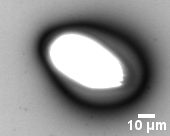
\includegraphics[width=4.0cm,height=4.0cm]{Figs/cuantificaciondefectos/hueco_cel_112.png}}{\caption{Defecto de superficie denominado agujero ó hueco, de (62.83 $\pm$0.59)$\mu$m de diámetro equivalente. }\label{fig:huecoazul}}
		\ffigbox{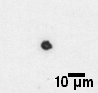
\includegraphics[width=4.0cm,height=4.0cm]{Figs/cuantificaciondefectos/mancha_cel_112.png}}{\caption{Defecto de superficie denominado mancha ó defecto de transmisión, de (6.33 $\pm$0.59)$\mu$m de diámetro equivalente.}\label{fig:manchaazul}}
	\end{floatrow}
\end{figure}

Los defectos de superficie de un componente óptico pueden estar originados en el proceso de fabricación mismo, en el tratamiento y manipulación de la óptica (en inglés, \textit{handling}) en distintas etapas de un proceso de montaje ó en el transporte del proveedor al cliente. Estos defectos pueden provocar un cambio de las propiedades ópticas del componente y en consecuencia los usuarios deben verificar la calidad óptica que los proveedores detallan en las especificaciones técnicas. A continuación se describen las dos especificaciones técnicas más utilizadas en la industria para determinar la calidad óptica de un componente, que son la \textit{U.S. Military Performance Specification} MIL-PRF-13830 y la ISO 10110 \cite{milprf}\cite{iso10110}. Ambas especificaciones fueron indicadas en la hoja de datos del filtro analizado en el presente trabajo.

\singlespacing
\subsection{MIL-PRF-13830: especificaciones de \textit{scratch \& dig}}
\label{sec:scanddig}
\spacing{1.5}

\hspace{0.5cm}La especificación técnica MIL-PRF-13830 define un \textit{scratch}(en adelante rayadura) como cualquier marca o rayadura de la superficie óptica del componente y un \textit{dig}(en adelante, simplemente defecto) como cualquier otro defecto de superficie presente en la óptica, como por ejemplo el agujero ó hueco de la Figura \ref{fig:huecoazul} ó el defecto de transmisión ó mancha de la Figura \ref{fig:manchaazul}. Esta reglamentación define las rayaduras y defectos permitidos en una superficie óptica utilizando una métrica dada por un par de números denominados \textit{scratch and dig numbers}: S/D. El \textit{scratch number} puede tomar alguno de los siguientes valores arbitrarios: 5,10,20,40,60,80, que representan en orden creciente el nivel de \underline{brillo} de la rayadura. Este número no proviene de una medición experimental exacta, sino que es el resultado de comparar el brillo de la rayadura del componente a analizar con muestras de rayaduras calibradas como las que se muestran esquemáticamente en la Figura \ref{fig:scratchanddig}, bajo ciertas condiciones de iluminación específicas (Ver \textit{Inspection method's}: 4.2.2.1 y 4.2.2. \cite{milprf}).
\begin{figure}[H]
	\centering
	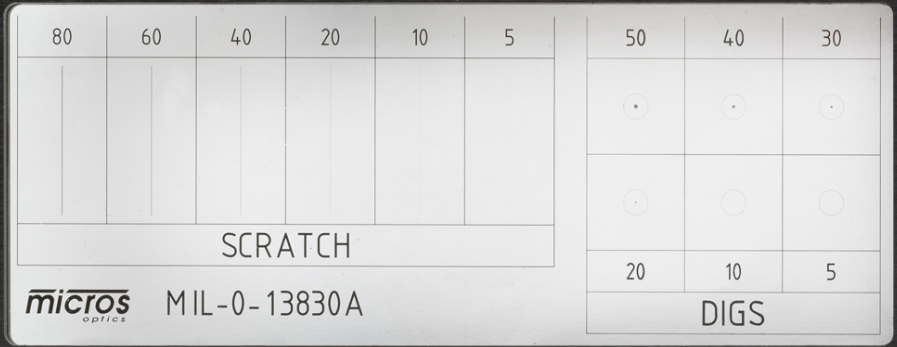
\includegraphics[scale=0.8]{Figs/cuantificaciondefectos/paddlecalibration.png}
	\caption{Muestra calibrada de \textit{scratch \& dig} comercializada por la empresa Thorlabs. Adaptado de \href{https://www.thorlabs.com/newgrouppage9.cfm?objectgroup_id=1427&pn=MOTP-MIL}{\texttt{https://bit.ly/3bPSMYS}}.}
	\label{fig:scratchanddig}
\end{figure}
El \textit{dig number} es el diámetro del defecto más grande permitido en el componente, dado en $1/100$ de milímetros. Por ejemplo, un componente con un \textit{dig number} de 40 implica que los defectos más grandes de la óptica pueden ser de un diámetro de hasta 0.2 mm. Si bien el \textit{dig number} es una cantidad medible experimentalmente con por ejemplo un microscopio, también se utilizan muestras calibradas para determinar el tamaño y cantidad de los defectos (Ver Figura \ref{fig:scratchanddig}). Luego de que un inspector entrenado cuantifica todas las rayaduras y defectos de la óptica con las muestras calibradas, se verifica la calidad óptica del componente de acuerdo a los siguientes criterios:
\begin{itemize}
\item La suma de todas las longitudes\footnote{La longitud es medida con una regla metálica (\textit{NIST traceable steel ruler}). En el caso de que la rayadura sea curva, su longitud es estimada por el inspector \cite{Aikens}.} de las rayaduras con el \textit{scratch number} (L$_{S_{\#}}$) asociado (máximo valor de brillo permitido) no podrá superar el valor de un cuarto del diámetro ($\Phi$) de la óptica. Si el componente no tuviera una geometría circular, se considera el diámetro de un círculo con un área igual al de la óptica bajo análisis.
\begin{equation}
\sum L_{S_{\#}} < \frac{\Phi}{4}
\label{eq:snumb}
\end{equation}
\item El número total (N) de defectos con el \textit{dig number} asociado (máximo diámetro de los defectos pemitido) no podrá exceder el diámetro de la óptica dividido por 20 mm. De obtenerse un número no entero, se trunca el resultado.
\begin{equation}
N  <  \frac{\Phi}{20 mm}
\label{eq:nphi20}
\end{equation}
\item La suma de todos los diámetros (d) de los defectos deberá ser menor ó igual al doble del número total de defectos de diámetro máximo permitido (N) multiplicado por el \textit{dig number} (D$_{\#}$) especificado en fracciones de milímetros.
\begin{equation}
\sum d 	\leq 2 . N . D_{\#}
\label{eq:dmenorig}
\end{equation}
\end{itemize}
\hspace{0.5cm}Así por ejemplo, una óptica de geometría circular con un diámetro de 200 mm y una calidad óptica especificada por el fabricante con \textit{scratch and dig numbers} S/D 30-20, puede tener rayaduras con un brillo calibrado de 30 y la suma de todas las longitudes de las rayaduras de brillo 30 no podrá ser superior a los 50 mm (de acuerdo a \eqref{eq:snumb}). Al mismo tiempo, la óptica no podrá tener más de 10 defectos de \textit{dig number} igual a 20, es decir de tamaño máximo de 0.2 mm (de acuerdo a  \eqref{eq:nphi20}) y la suma de los diámetros de todos los defectos no podrá ser superior a los 4 mm (de acuerdo a \eqref{eq:dmenorig}).

La Figura \ref{fig:samplescratchs} muestra una comparación de cuatro muestras de calibración de rayaduras, medidas bajo idénticas condiciones de iluminación \cite{Aikens}.
\begin{figure}[H]
	\centering
	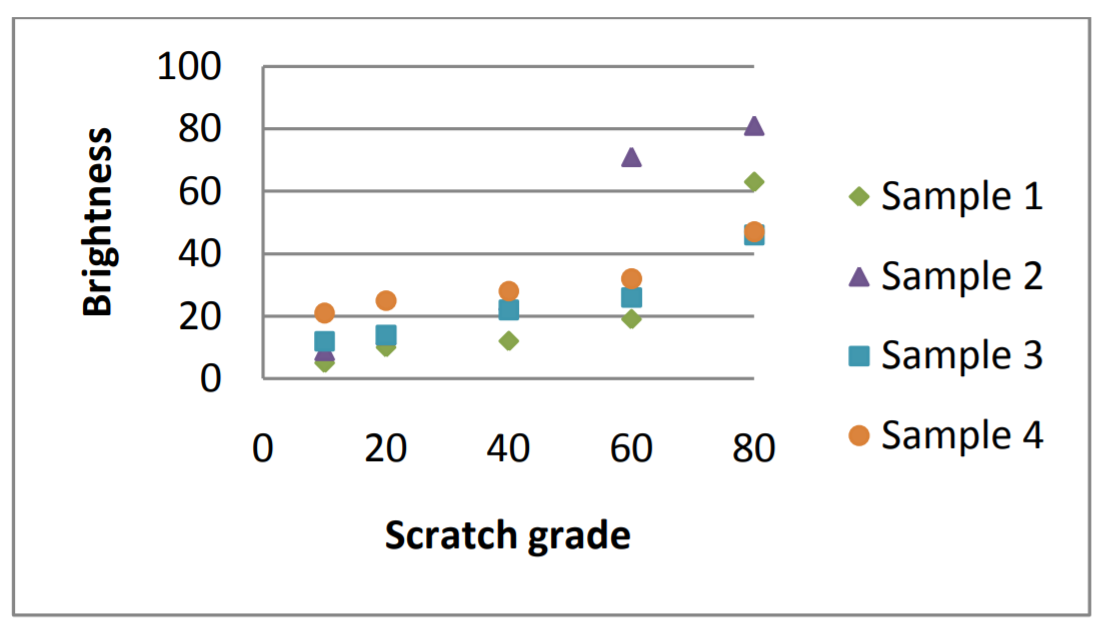
\includegraphics[scale=0.54]{Figs/cuantificaciondefectos/samplesscratch.png}
	\caption{Brillo relativo de cuatro muestras calibradas de \textit{scratch number}. \textit{Sample} en inglés significa muestra. La muestra 1 es de la empresa FLIR/Brysen (S\&D 1109), la muestra 2 es de Davidson Optronics (D-667A S/N 2431), la muestra 3 es de Eastman Kodak (\textit{paddle} EKCO CM2) y la muestra 4 es de Jenoptik (\textit{paddle} EO \#53-157 CM1). La muestra 4 es vendida comercialmente por los proveedores Edmund Optics y por Thorlabs. Gráfico tomado de \cite{Aikens}.}
	\label{fig:samplescratchs}
\end{figure}


De la Figura \ref{fig:samplescratchs} se desprende que las cuatro muestras son incompatibles entre sí, es decir arrojan resultados de brillo distintos entre sí para un cierto \textit{scratch number}. Se observa que para un \textit{scratch number} igual a 10, el brillo de la muestra 4 es de mayor intensidad que el \textit{scratch number} 60 de la muestra 1.
Así también el brillo del \textit{scratch number} 60 de la muestra 2 es más de dos veces más brillante que cualquiera de las otras muestras para este mismo \textit{scratch number}.

Además, la métrica de \textit{scratch \& dig} tiene la falencia de no poder caracterizar ni rayaduras de brillo menores al \textit{scratch number} igual a 5 ni defectos con un \textit{dig number} menor a 5, es decir que no se consideran defectos de diámetro menores a los 50 $\mu m$ \cite{quentin}. Esto es así pues esos números de \textit{scratch \& dig} son los valores más chicos presentes en las muestras calibradas para la inspección visual de acuerdo a los dibujos técnicos oficiales de la métrica(Ver \cite{dibujito})  .

Si bien la métrica de \textit{scratch and dig} sigue siendo ampliamente utilizada en la industria, el hecho de que el análisis de las rayaduras y defectos sea dependiente del inspector de turno sumado a que las muestras de brillo calibradas varían de acuerdo al fabricante de las mismas y que sólo sean considerados defectos con un diámetro mínimo de 50 $\mu m$, hacen que esta especificación técnica para determinar la calidad de una óptica resulte técnicamente ambigua e imprecisa.  A continuación se explican las especificaciones técnicas de la ISO 10110. Luego se muestran las características del filtro analizado en esta tesis junto a sus especificaciones ópticas de calidad.

\singlespacing
\subsection{ISO 10110-7: defectos de superficie}
\label{sec:iso10110}
\spacing{1.5}


\hspace{0.5cm}Las tolerancias de la normativa ISO 10110 vienen dadas por el número de defectos permitidos ($N_{p}$) y por un coeficiente dado en fracciones de milímetros denominado \textit{grade number} ($A_{g}$) que es igual a la raíz cuadrada del área del defecto de diámetro máximo permitido. Estos dos valores son expresados en las hojas de datos de los componentes ópticos de la siguiente manera: 5/$N_{p}$x$A_{g}$. El número 5 hace referencia a que la especificación técnica dada se refiere a las tolerancias de los defectos de superficie (Parte 7 de la ISO 10110). 

Se hace notar que si no es especificado en la hoja de datos del componente, el \textit{grade number} incluye a cualquier tipo de defectos, rayaduras, etc y en ese sentido evita la ambiguedad de la comparación con las muestras calibradas de \underline{brillo} de las rayaduras. Ahora bien, la normativa establece que el control de calidad de los componentes puede ser realizado por inspección visual con muestras calibradas de defectos con distintos \textit{grade numbers}(Ver \href{https://www.thorlabs.com/thorproduct.cfm?partnumber=MOTP-ISO}{MOTP-ISO} ó \href{https://www.edmundoptics.com/p/scratch-amp-dig-target-1st-surface-positive/15899/}{EO \# 59-154}) y también incluye a la inspección automatizada de los defectos lo que resulta una novedad respecto de la normativa anterior. Sin embargo, de realizarse esto último la reglamentación establece que tiene que haber un acuerdo entre el fabricante y el cliente y que el equipamiento utilizado y las condiciones experimentales específicas para realizar el control de calidad tienen que estar especificadas en la hoja de datos del componente bajo análisis \cite{acuerdocon}.

Ahora bien, un componente óptico supera las especificaciones de la ISO 10110 mediante el método de inspección visual si supera las siguientes condiciones:
\begin{itemize}
\item No pueden existir defectos con un \textit{grade number} mayor al especificado en la hoja de datos del componente.
\item El área del componente óptico cubierta por defectos `relevantes'\footnote{Por defectos `relevantes' se considera a los defectos de \textit{grade number} mayor al defecto de mínimo \textit{grade number} detectado vía inspección visual. De acuerdo a la ISO 14997 que es una implementación de los métodos de control de calidad especificados por la ISO 10110-7, el \textit{grade number} del defecto más chico a considerar vía la inspección visual es de un \textit{grade number} igual a 0.040 (40 $\mu m$ de diámetro) \cite{etsol}.} ($A_{defectos}$) no puede superar el valor de la siguiente expresión:
\begin{equation}
A_{defectos} = N_{p}\hspace{2pt} .\hspace{2pt} A_{g}^{2}
\label{eq:isoarea}
\end{equation}
\end{itemize}
\hspace{0.5cm}Por ejemplo, la especificación 5/5x0.05 brindada por un cierto fabricante, indica que el componente cumple que tiene como máximo 5 defectos de \textit{grade number} igual a 0.05 (diámetro de 50 micrones) y el área máxima cubierta por los defectos con un \textit{grade number} mayor ó igual a 0.04 puede ser de 12500 $\mu m^{2}$.

 En esta sección se definió el concepto de defecto de superficie de un componente óptico como cualquier inhomogeneidad presente en la superficie bajo análisis. Se describieron las dos especificaciones técnicas más utilizadas para determinar la calidad óptica de la superficie de un componente, ambas presentes en la hoja de datos del filtro a analizar en la presente tesis. Por un lado, las especificaciones de \textit{scratch \& dig} que resultan un poco ambiguas debido a la determinación subjetiva de los \textit{scratch numbers} del componente. Y, por otro lado, la ISO 10110 que propone superar esta ambiguedad no distinguiendo los tipos de defectos presentes en la óptica, sino tratándolos a todos por defectos en general por igual. En cualquier caso se hace notar que el control de calidad del componente óptico de interés por parte del cliente tiene que ser realizado bajo las mismas condiciones experimentales y utilizando el mismo criterio (teniendo un total acuerdo en la letra chica de cualquier especificación) que el proveedor.
 
 A continuación se describen las características y dimensiones del filtro analizado en este trabajo y luego se describe el método de inspección del filtro implementado a partir de la adquisición de imágenes por transmisión con un microscopio.

\singlespacing
\section{Características del filtro}
\label{sec:carfilt}
\spacing{1.5}

\hspace{0.5cm}El componente óptico analizado en la presente tesis, denominado en adelante simplemente filtro, consiste de un arreglo de cinco filtros ópticos de interferencia  considerados en adelante a cada uno de ellos como una banda. En la Figura \ref{fig:filtroposta} se muestra el filtro real analizado y en la Figura \ref{fig:dimsfiltr} se muestran las diimensiones especificadas por el fabricante.
\begin{figure}[H]
	\begin{floatrow}
		\ffigbox{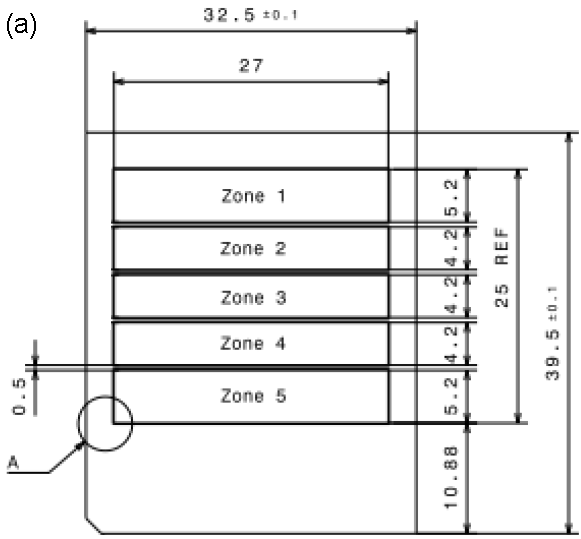
\includegraphics[scale=0.8]{Figs/cuantificaciondefectos/dimsfiltro.png}}{\caption{Dimensiones del filtro especificadas por el fabricante.}\label{fig:dimsfiltr}}
		\ffigbox{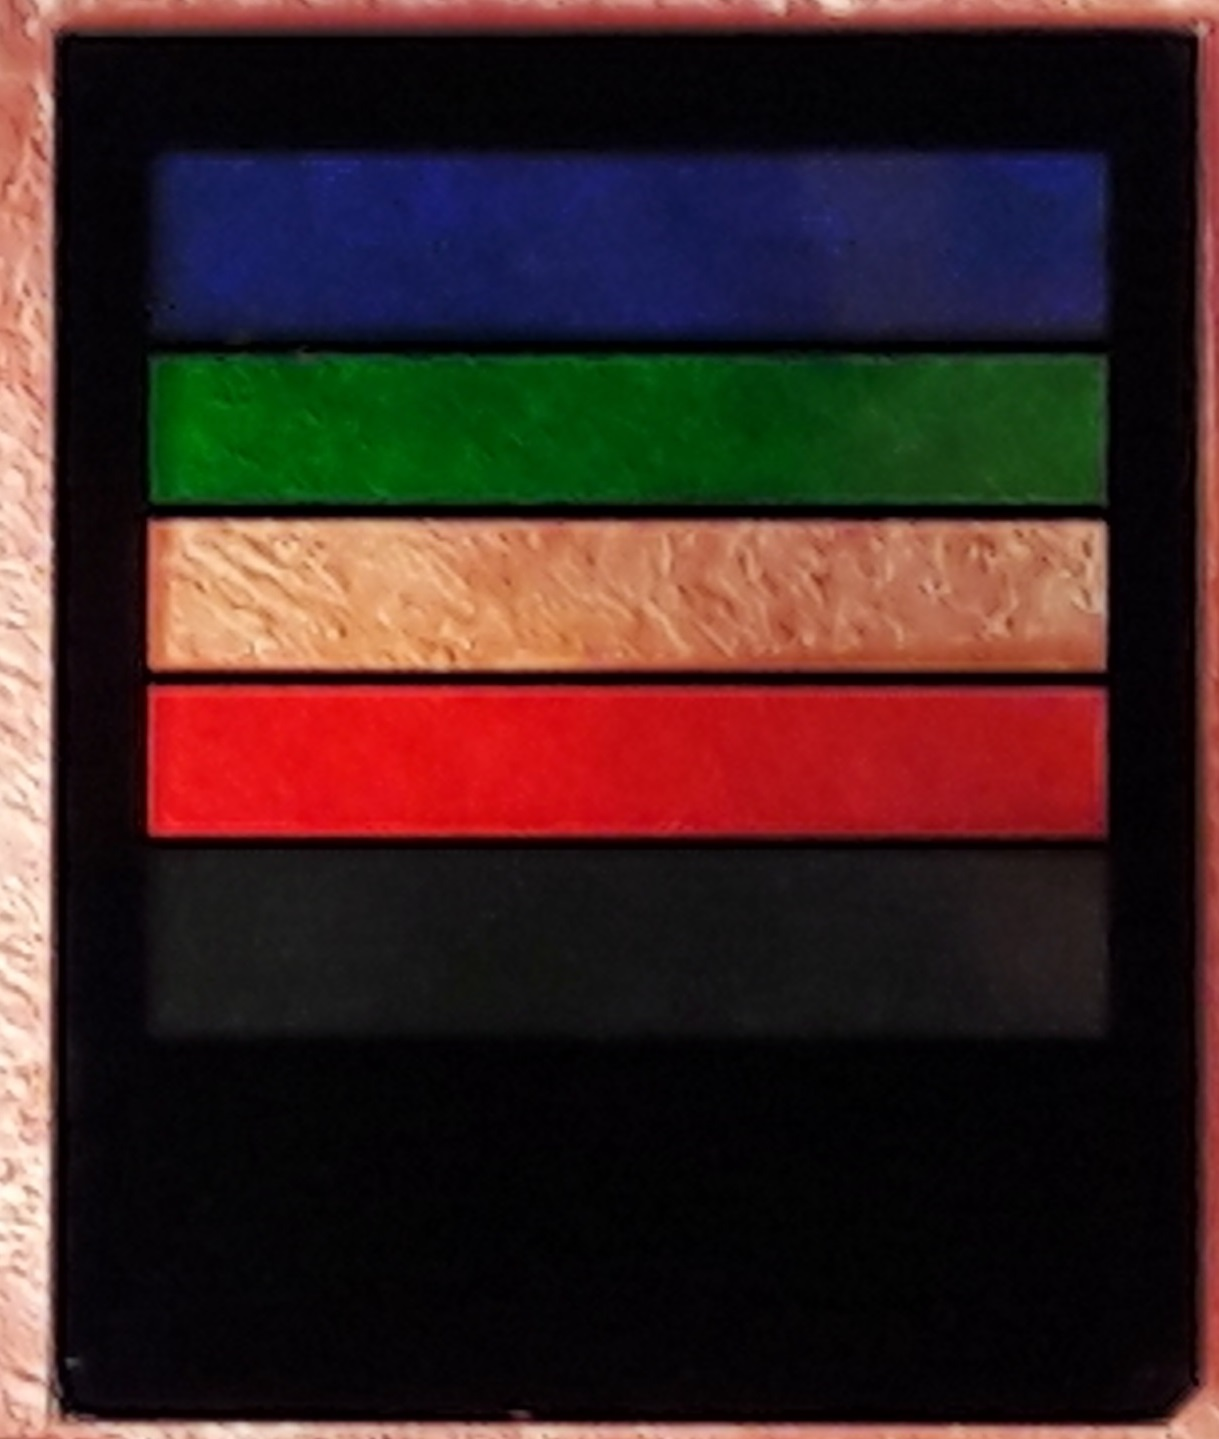
\includegraphics[scale=0.15]{Figs/cuantificaciondefectos/filtro_real.jpg}}{\caption{Imagen del filtro real analizado.}\label{fig:filtroposta}}
	\end{floatrow}
\end{figure}
Las zonas (en inglés, \textit{zone}) están asociadas a una cierta banda espectral de transmisión de la siguiente manera:
\begin{itemize}
\justifying
\item Zona 1 - Banda Azul: (450-510) nm
\item Zona 2 - Banda Verde: (510-580) nm
\item Zona 3 - Banda Pancromática\footnote{La palabra pancromática, del griego ático donde pan significa todo y cromático viene de la familia de la palabra color, implica que dicha banda tiene un espectro de transmisión en toda la región del visible.}: (450-750) nm
\item Zona 4 - Banda Roja: (590-690) nm
\item Zona 5 - Banda NIR\footnote{NIR, en inglés \textit{Near-Infrared}, se le denomina a la región espectral del infrarrojo cercano que se extiende aproximadamente desde los 780 nm hasta los 2000 nm.}: (750-900) nm
\end{itemize}
 \hspace{0.5cm}Las especificaciones ópticas de calidad de \underline{cada banda} del filtro brindadas por el fabricante son las siguientes:
\begin{center}
5/2x0.063 (\textit{according to MIL PRF 13830, S/D 20-10})
\end{center}
\hspace{0.5cm}Estas especificaciones implican para el caso de la ISO 10110, 5/2x0.063, que en la superficie óptica de \underline{cada banda} puede haber un máximo de 2 defectos de \textit{grade number} igual a 0.063 (63 $\mu m$ de diámetro), que no puede haber defectos con un \textit{grade number} mayor a 0.063 y que el área total máxima cubierta por defectos de \textit{grade number} mayor a 0.04 (diámetro de 40 $\mu m$) puede ser de 7938 $\mu m^{2}$, de acuerdo a \ref{eq:isoarea}. Y, las especificaciones de \textit{scratch \& dig}, S/D 20-10, indican que en cada banda puede haber rayaduras con un brillo calibrado de \textit{scratch number} igual 20 y que la suma de todas las longitudes de las rayaduras del mismo valor de \textit{scratch number} no podrá ser superior al diámetro equivalente de cada banda, de acuerdo a \ref{eq:snumb}. Por último, cada banda del filtro no deberá tener más de 1 defecto de \textit{dig number} igual a 10 (diámetro de 100 $\mu m$)  de acuerdo a \ref{eq:nphi20}\footnote{Las dimensiones de la banda más chica son de 4.2 mm x 27.0 mm con lo cual el diámetro equivalente es de 12.0 mm. El cociente de la Ecuación \ref{eq:nphi20} es igual a 0.6, resultado que se trunca a 1. El resultado final es el mismo para todas las bandas.}  y la suma de los diámetros de todos los defectos no podrá ser superior a los 0.2 mm, de acuerdo a \ref{eq:dmenorig}. 

El fabricante no aclaró el método de inspección utilizado para garantizar la calidad óptica especificada del filtro de la \underline{normativa ISO 10110}. Ahora bien, el fabricante indica en su página \textit{web} que realiza una inspección visual con muestras calibradas para garantizar la calidad óptica de sus componentes con lo cual en la presente tesis se va a suponer que dicha especificación fue realizada a través de ese método únicamente.

Se hace notar que entre las bandas se encuentran unas regiones rectangulares de cromo, de $(0.5 \pm 0.1)mm $ de largo como se muestra en la Figura \ref{fig:dimsfiltr}. El mismo material cubre toda la región del filtro no contenida por las cinco bandas.

A continuación se describe el proceso de adquisición de las imágenes del filtro, posteriormente su procesamiento y el algoritmo de detección de los defectos y por último se discute un análisis cuantitativo de los mismos.

\singlespacing
\section{Adquisición de las imágenes del filtro}
\label{sec:conf}
\spacing{1.5}

\hspace{0.5cm}Con el propósito de cuantificar y caracterizar los defectos del filtro se adquirieron imágenes micróscopicas del mismo. Para la adquisición de las imágenes se utilizó un microscopio invertido Zeiss Axio Observer Z1 como se muestra en la Figura \ref{fig:ZEISSdellabo}, con un objetivo Zeiss N-Achroplan de magnificación 10X y apertura numérica de 0.25.
\begin{figure}[H]
	\centering
	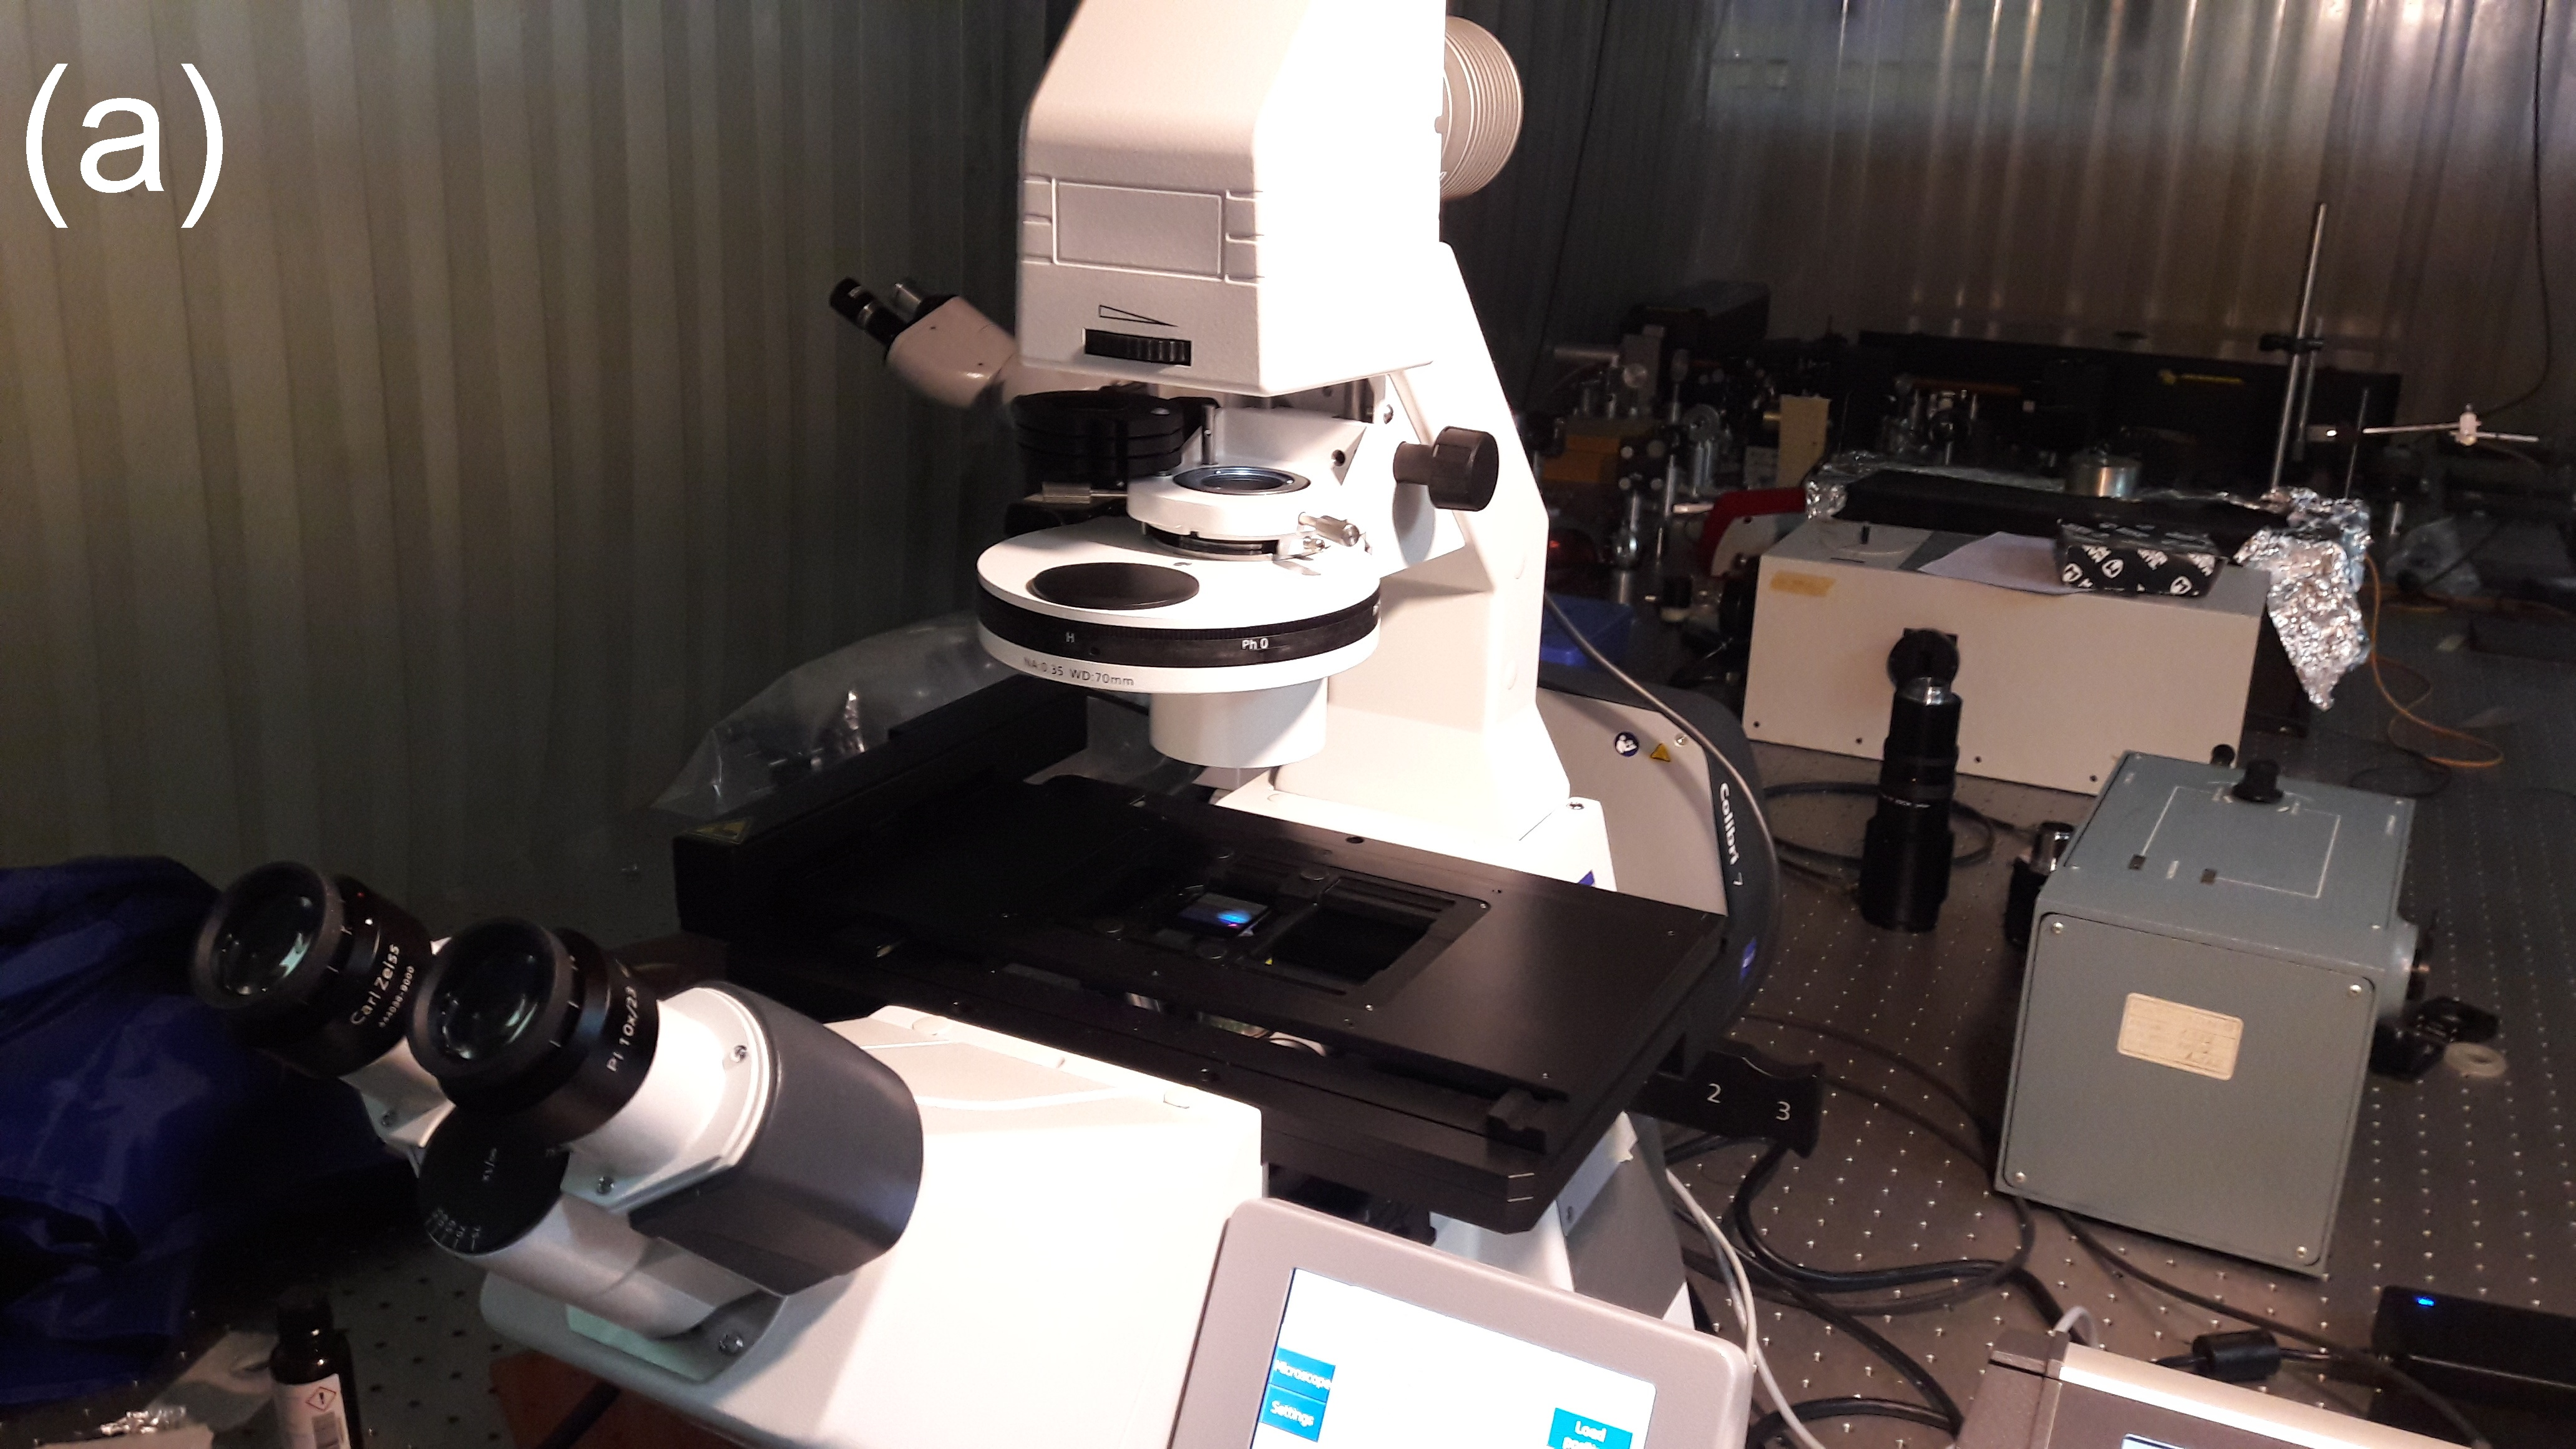
\includegraphics[scale=0.1]{Figs/defectosZEISS/b.jpg}
	\caption{Microscopio invertido Zeiss Axio Observer Z1.}
	\label{fig:ZEISSdellabo}
\end{figure}

Las imágenes del filtro fueron adquiridas por transmisión utilizando una fuente de luz blanca, en condiciones de \textit{bright field}\footnote{Técnica de iluminación que en castellano suele ser denominada de 'campo brillante' para diferenciarla de la iluminación de campo oscuro (en inglés \textit{dark field}, ver \href{https://es.wikipedia.org/wiki/Microscopio_de_campo_oscuro}{\faWikipediaW}).}. Se montó el filtro sobre el portamuestras de la platina del microscopio como se muestra en la Figura \ref{fig:filtroenZEISS} y mirando por el ocular se puso en foco la superficie del filtro a medir.  
\begin{figure}[H]
	\centering
	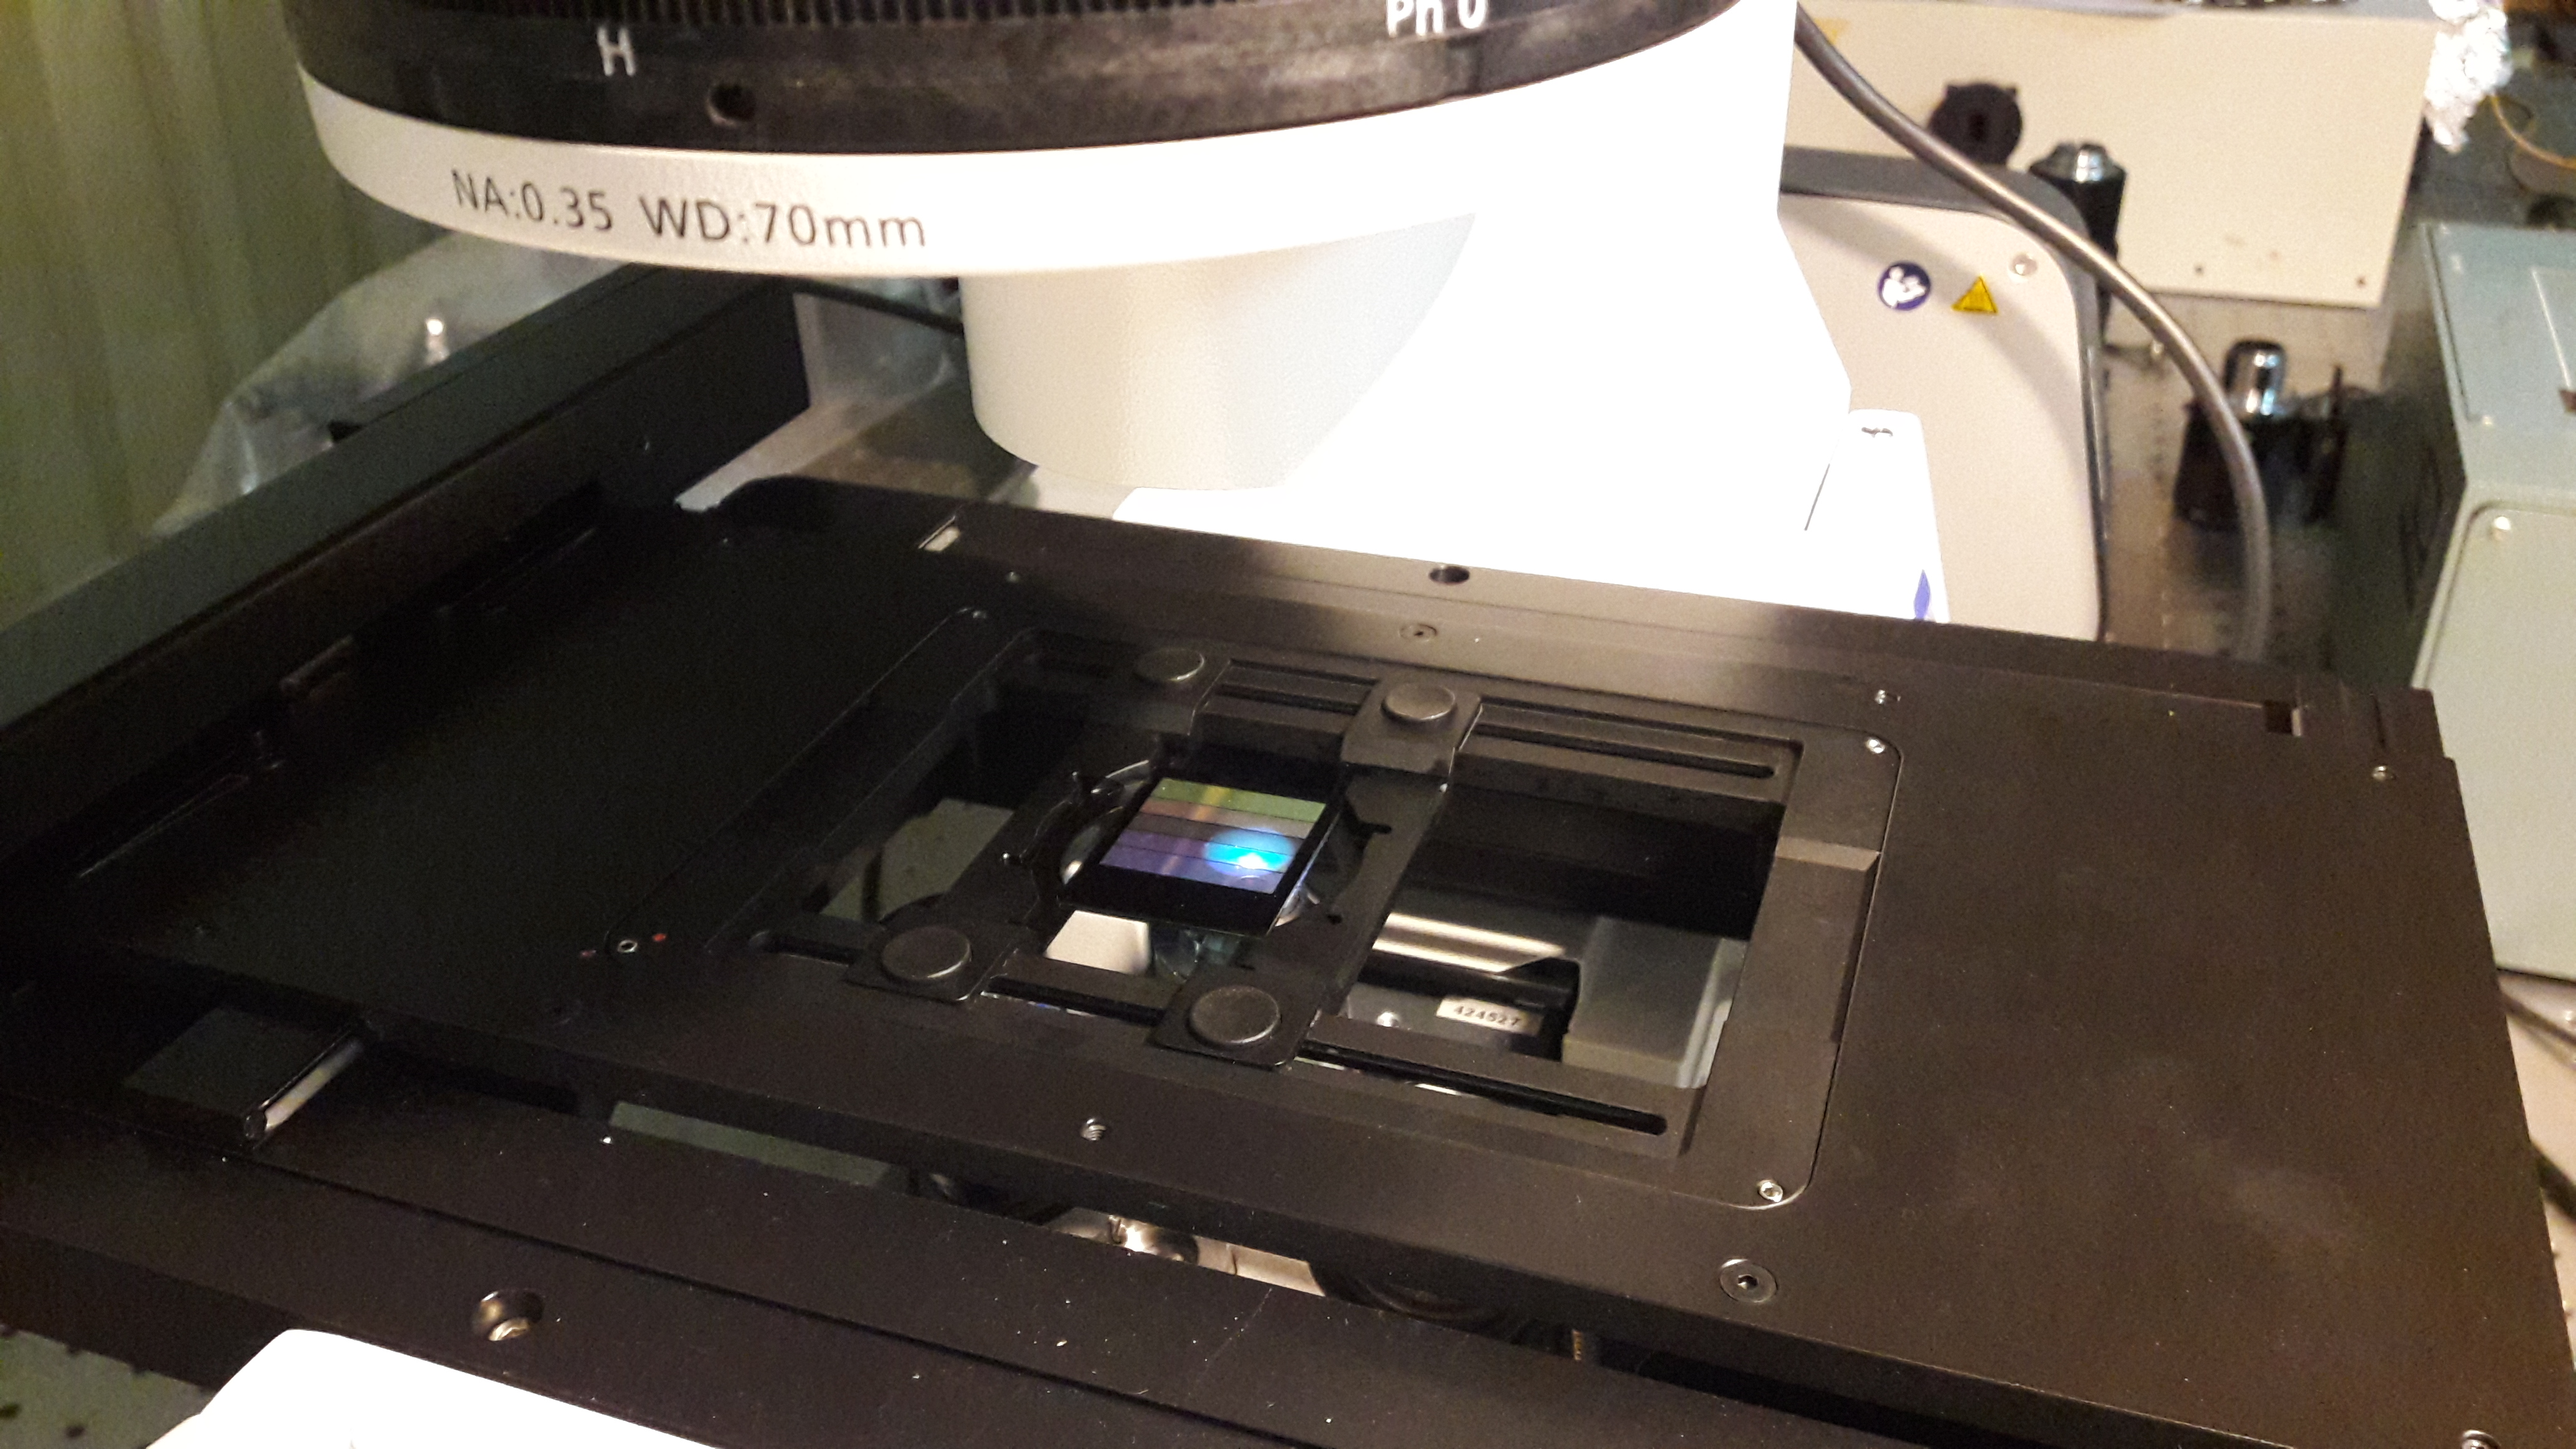
\includegraphics[scale=0.1]{Figs/defectosZEISS/a.jpg}
	\caption{Montaje del filtro sobre el portamuestras de la platina del microscopio.}
	\label{fig:filtroenZEISS}
\end{figure}
La cámara monocromática del microscopio del fabricante Zeiss, modelo Axiocam 702, con un sensor CMOS de 1/1.2'' (diagonal de 13.3mm) y una resolución de 2.3 megapíxeles (1216x1920 píxeles), fue controlada a través del software ZEN 2.5 (\textit{Blue edition}, 2018) del mismo fabricante. Se utilizó la calibración de la cámara que viene de fábrica del microscopio para la configuración utilizada, donde 1 píxel equivale a 0.586 $\mu m$.  Cada \textit{tile} individual tiene las dimensiones del \textit{field of view} (FOV\footnote{En castellano es el campo de visión y representa el área física de la imagen, que para el caso de una cámara el FOV viene dado por el cociente entre el tamaño del sensor CMOS y la magnificación del microscopio.}) de la cámara, que son de 713 $\mu m$ x 1125 $\mu m$. 

Se configuró el software para adquirir las imágenes por transmisión, en particular se eligió la fuente de luz blanca y para cada medición su intensidad, además del tiempo de exposición de la cámara. Como la cámara tiene otro arreglo óptico que el ocular, el plano focal de la superficie del filtro elegida para medir se encuentra a una distancia distinta entre el objetivo y la muestra. En consecuencia, con las perillas manuales del microscopio se pone en foco la imagen observando la adquisición en vivo en la computadora. 


\singlespacing
\subsection{\textit{Tile scan}}
\spacing{1.5}

\hspace{0.5cm}A continuación se explica cómo se adquirieron las imágenes para una determinada región del filtro, ya sea para el filtro completo a excepción de la banda del NIR ó para cada banda espectral del filtro en particular.

La palabra en inglés \textit{tile} significa baldosa en castellano y realizar un \textit{tile scan} implica realizar un barrido de adquisición de imágenes de una cierta área a elección de una muestra donde el área total a adquirir está compuesta por múltiples baldosas. Cada baldosa, es decir cada \textit{tile} constituye una imagen del microscopio de acuerdo al \textit{field of view} (FOV) que se tiene del arreglo óptico de la cámara integrada al microscopio. En la Figura \ref{fig:tilescan} se muestra un ejemplo de un \textit{tile scan} de la banda pancromática del filtro.

Existen distintas formas de elegir el área total a adquirir en el software. Se eligió la opción de determinar la región a adquirir a partir de la selección visual individual de las cuatro esquinas de la misma, es decir las posiciones [0,0],[xf,0],[0,yf], [xf,yf] de acuerdo al sistema de coordenadas de la Figura \ref{fig:tilescan}. Para elegir estas esquinas el microscopio cuenta con un \textit{joystick} que permite mover la platina motorizada del microscopio en el plano de la imagen y se tiene activada la adquisición en vivo en el software ZEN para elegirlas visualmente.


\begin{figure}[H]
	\centering
	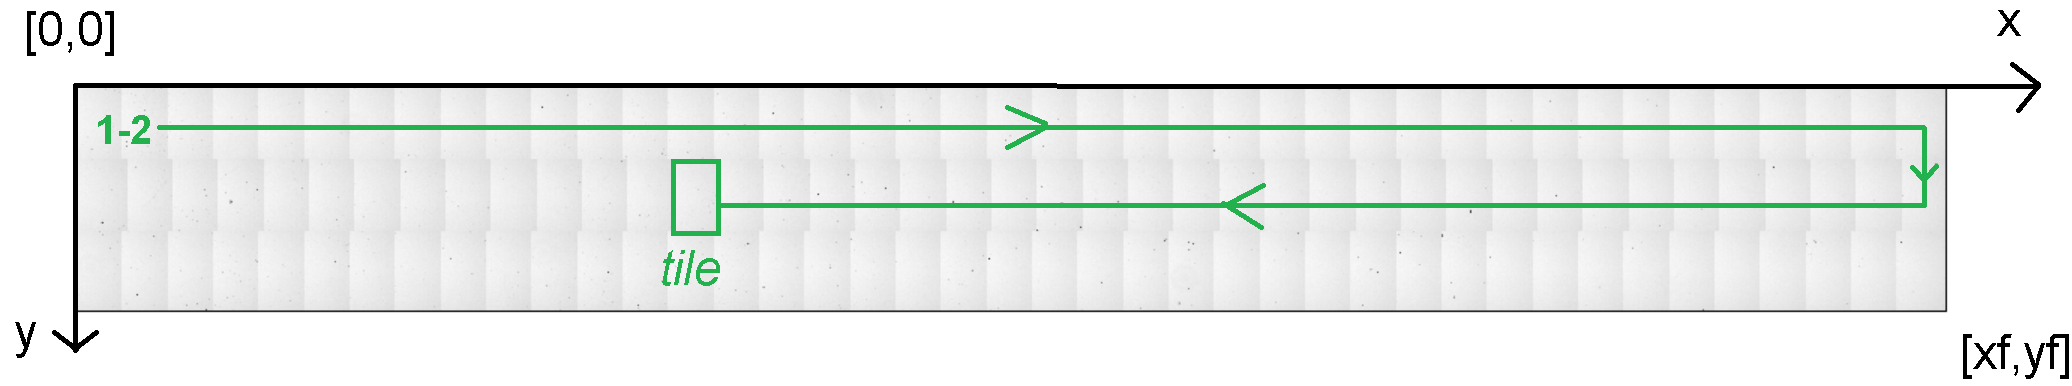
\includegraphics[width=1.0\textwidth]{Figs/cuantificaciondefectos/tilescan.png}
	\caption{\textit{Tile scan} de la banda pancromática.}
	\label{fig:tilescan}
\end{figure} 

Cada trayectoria del barrido fue realizada automáticamente de la siguiente manera: la platina motorizada se posicionó en el centro del FOV de la primera \textit{tile} a adquirir asociada a las coordenadas [0,0] de la imagen de la Figura \ref{fig:tilescan} y se adquirió la primera imagen individual del barrido completo de la región a adquirir, en este ejemplo la banda pancromática. A continuación la platina motorizada se desplazó en el sentido definido positivo del eje x hasta el centro del FOV de la segunda \textit{tile} a adquirir teniendo en cuenta el \textit{overlap} configurado y así siguiendo una trayectoria que barre por `filas' completas a lo largo del eje x que van variando con el desplazamiento discreto vertical en el eje y cuando se llega a los extremos del eje x.

Entre otros parámetros del barrido, se eligió el \textit{overlap} entre las baldosas, es decir la superposición entre las mismas que luego permite obtener una imagen completa individual para su \underline{visualización},  realizando un \textit{stitching}\footnote{El \textit{stitching} es el proceso computacional por el cual se combinan múltiples \textit{tiles} para
producir una sola imagen que permita una mejor visualización (Ver técnica SIFT (\textit{Scale Invariant Feature Transform}), \cite{Lowe}).} como post-procesamiento de las imágenes. Este último procedimiento también fue realizado con el software de Zeiss. Se configuró el \textit{overlap} en 10$\%$ para todas las mediciones, siendo este valor el mínimo encontrado para que el \textit{stitching} entre las imágenes consecutivas sea realizado correctamente sin dejar espacios en blanco y para que dicha superposición elimine de la imagen la menor cantidad de defectos posibles. Por último, se elige en la configuración que cada baldosa de la región barrida sea exportada como una imagen individual para su posterior \underline{análisis}.

\singlespacing
\subsection{Superficies y mapa de los defectos del filtro}
\spacing{1.5}

\hspace{0.5cm}Se adquirieron imágenes completas del filtro, a excepción de la banda espectral del NIR, para las dos superficies exteriores del filtro como se muestra en las Figuras \ref{fig:supfiltrocondensador} y \ref{fig:supfiltroobjetivo}.
\begin{figure}[H]
	\begin{floatrow}
		\ffigbox{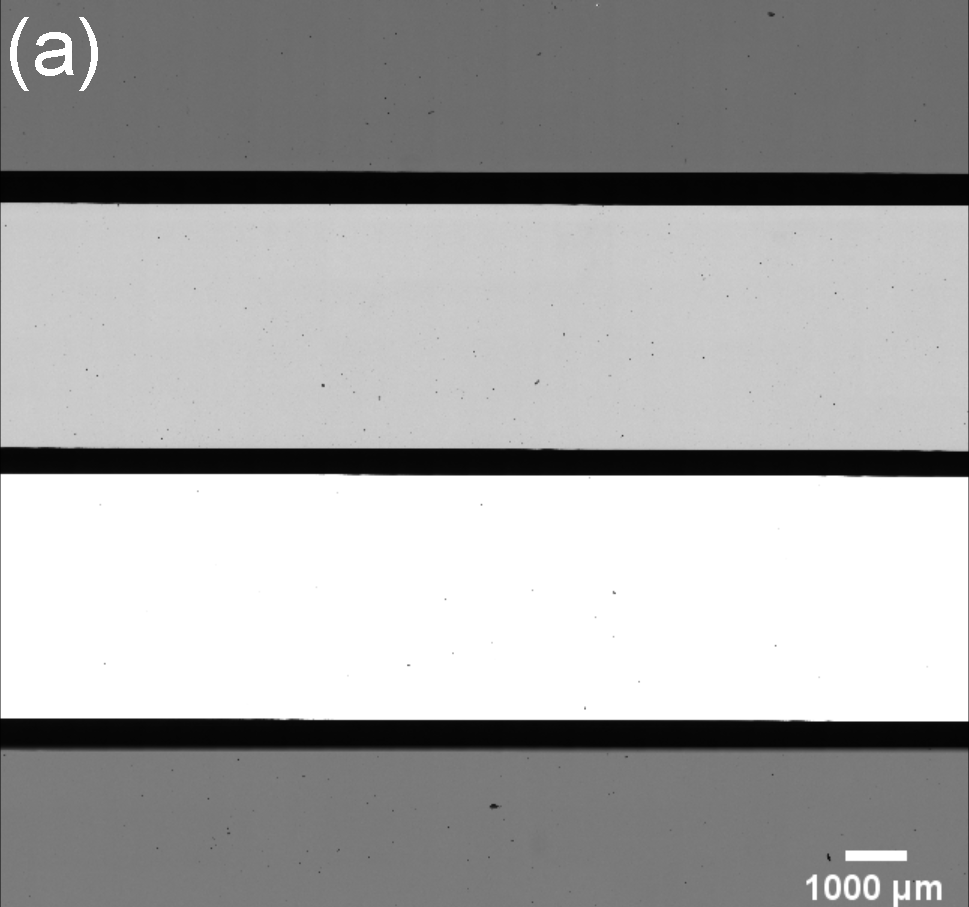
\includegraphics[width=7.5cm,height=7.33cm]{Figs/cuantificaciondefectos/supextex2216.png}}{\caption{Imagen de la superficie exterior A del filtro, para un barrido de 15.54 mm x 14.94 m.}\label{fig:supfiltrocondensador}}
		\ffigbox{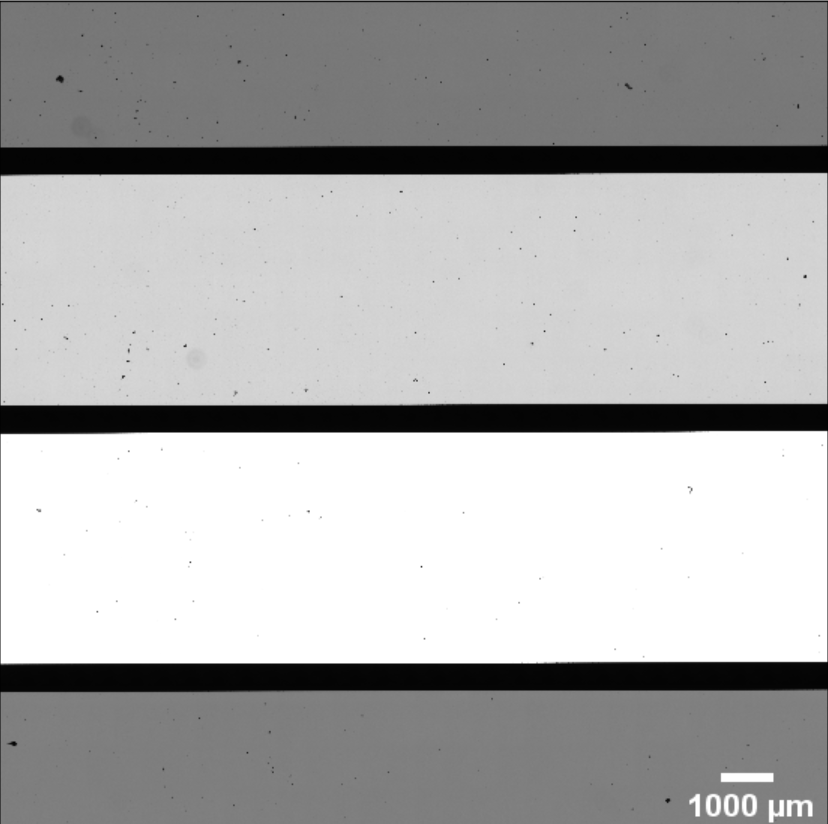
\includegraphics[width=7.5cm,height=7.33cm]{Figs/cuantificaciondefectos/supextex1515.png}}{\caption{Imagen de la superficie exterior B del filtro, para un barrido de 15.50 mm x 15.55 mm.}\label{fig:supfiltroobjetivo}}
	\end{floatrow}
\end{figure}
 Las dos superficies exteriores denominadas arbitrariamente A y B son las que se muestran especificadas en la Figura \ref{fig:espfil} y que se encuentran en la interfaz filtro-aire. En las Figuras \ref{fig:supfiltrocondensador} y \ref{fig:supfiltroobjetivo} se muestran las bandas espectrales del filtro en orden descendente: Azul (450-510 nm), Verde (510-580 nm), Pancromática (450-750 nm), Roja (590-690 nm). El brillo, el contraste y el tamaño de las imágenes originales fueron modificados para obtener una mejor visualización, utilizando el software FIJI-ImageJ. 
\begin{figure}[H]
	\centering
	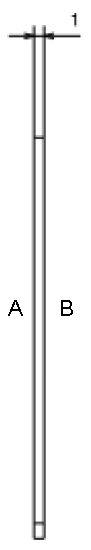
\includegraphics[scale=0.4]{Figs/cuantificaciondefectos/espesorfiltro.png}
	\caption{Dimensiones del espesor del filtro: (1.0 $\pm$ 0.1)mm. Las superficies exteriores del filtro son las superficies A y B, que se encuentran en la interfaz filtro-aire.}
	\label{fig:espfil}
\end{figure}
Para realizar el barrido completo de cada superficie se verificó en las cuatro esquinas de la superficie a medir que no se pierda el foco de la imagen. Se eligió la intensidad de la fuente de luz y el tiempo de integración de la cámara tales que no sature alguna de las bandas del filtro de forma tal poder adquirir una imagen completa del filtro en un solo barrido, y de forma tal que se utilice la mayor parte del rango dinámico de la cámara, como se puede ver en el histograma de la intensidad de los píxeles de la Figura \ref{fig:histograma15x15} para el barrido de la superficie A del filtro. 
\begin{figure}[H]
	\centering
	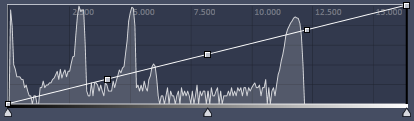
\includegraphics[width=1.0\textwidth]{Figs/defectosZEISS/histograma15x15.png}
	\caption{Histograma de la intensidad de los píxeles de la cámara del barrido de la superficie exterior A del filtro que se observa en el software ZEN del microscopio.}
	\label{fig:histograma15x15}
\end{figure}
Se hace notar que la banda del NIR no pudo ser adquirida en el barrido completo de las superficies exteriores del filtro pues con los valores de intensidad de la lámpara y del tiempo de adquisición de la cámara fijados para que ninguna de las bandas del filtro sature, no era posible obtener una imagen de esa banda. Si bien la cámara tiene un rango de sensibilidad espectral comprendido entre los 350 nm y los 1000 nm de acuerdo a su hoja de datos \cite{axiozeiss}, del gráfico de la eficiencia cuántica\footnote{La eficiencia cuántica, en inglés \textit{Quantum efficiency} (QE), es una medida precisa de la sensibilidad de un dispositivo fotosensible que permite determinar como es la respuesta del dispositivo para cada longitud de onda.} se desprende que para la región espectral del NIR tiene una eficiencia cuántica menor al 30\% (Ver Figura \ref{fig:eficienciacuanticamara}). A esto se le suma el hecho de que la fuente de luz tiene un espectro de emisión centrada en el ultravioleta y con una fuerte componente del espectro visible pero de relativa poca intensidad en la región del NIR, como se muestra en el gráfico de la intensidad en función de la longitud de onda de la Figura \ref{fig:espectrolamparazeiss}. Dicho espectro fue medido con el espectrómetro CCS200 de Thorlabs. 
\begin{figure}[H]
	\centering
	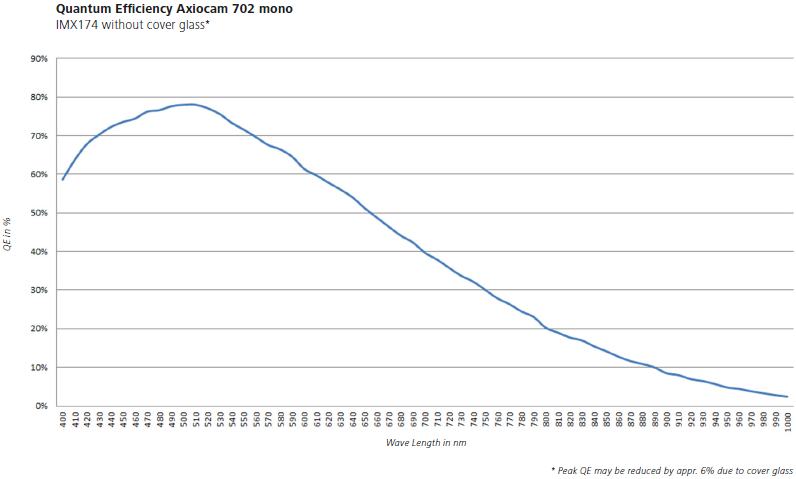
\includegraphics[width=1.0\textwidth]{Figs/defectosZEISS/eficienciacuanticacamarazeiss.png}
	\caption{Gráfico de la eficiencia cuántica de la cámara monocromática del microscopio Aiocam 702 en función de la longitud de onda.}
	\label{fig:eficienciacuanticamara}
\end{figure}
\begin{figure}[H]
	\centering
	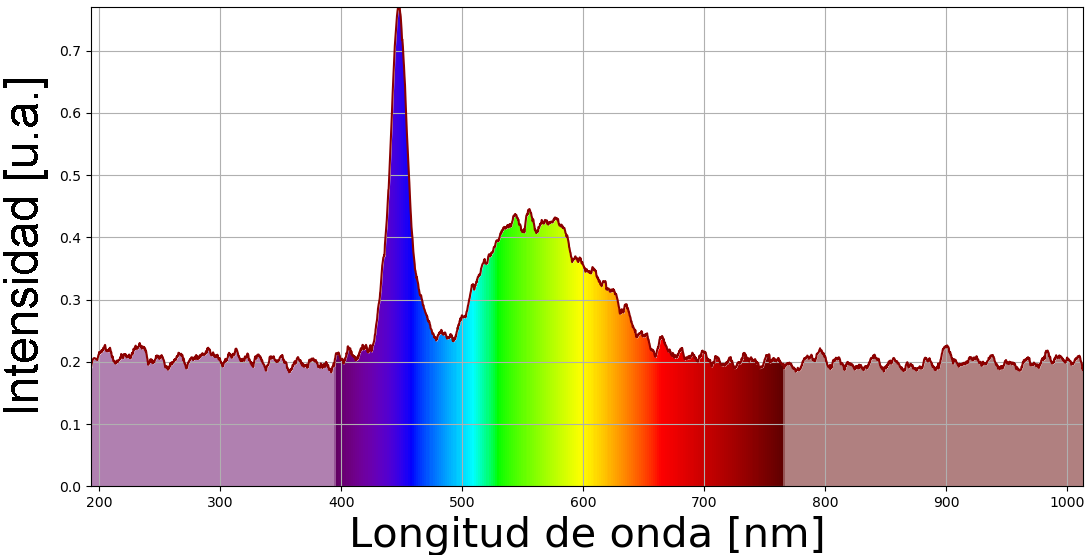
\includegraphics[width=1.0\textwidth]{Figs/defectosZEISS/espectrolampZEISSacolor.png}
	\caption{Espectro de emisión de la fuente de luz del microscopio.}
	\label{fig:espectrolamparazeiss}
\end{figure}

Ahora bien, la banda espectral del NIR fue medida individualmente posteriormente como se explica más adelante. Para poder obtener una imagen del filtro completo, incluida la banda del NIR, se debería cambiar la fuente de luz por una que tenga una mayor intensidad en dicha región espectral.

La imagen completa de cada superficie exterior del filtro permitió:
\begin{itemize}
	\item Realizar un primer diagnóstico visual general por imagen de la calidad óptica de construcción del filtro. 
	\item Determinar que ninguna de las dos superficies exteriores del filtro presentaba una cantidad mayor notable de defectos que la otra como se puede observar en las Figuras \ref{fig:supfiltrocondensador} y \ref{fig:supfiltroobjetivo}, por lo que el análisis individual de cada una de las bandas fue realizado sobre una de las caras únicamente.
	\item Obtener un mapa de los defectos con su ubicación precisa en la superficie del filtro para ser utilizado luego con el microespectrómetro (Ver Capítulo \ref{chap:microsp}).
\end{itemize}

A continuación se explica el proceso de adquisición de las imágenes individuales de cada banda espectral, el pre-procesamiento de las mismas que consiste en la corrección de la iluminación no uniforme del microscopio y luego se describe el algoritmo de detección de los defectos.

\singlespacing
\subsection{Adquisición de imágenes individuales de cada banda espectral}
\spacing{1.5}

\hspace{0.5cm}Para realizar una cuantificación de los defectos del filtro, se adquirieron imágenes individuales de cada banda espectral del filtro para una de las superficies exteriores del filtro. Para cada banda, se configuró la intensidad de la lámpara y el tiempo de integración de la cámara de forma tal de utilizar la mayor parte del rango dinámico de la cámara que se encuentra alrededor del 70 \% recomendado por el fabricante y de esta forma obtener la mejor calidad de imagen para el posterior análisis de cada banda. Así también se verificó que las cuatro esquinas de la banda a medir estuvieran en foco a partir de la visualización en vivo de la cámara. Dichas esquinas fueron elegidas en el software para determinar el área a ser barrida con el \textit{tile scan} teniendo cuidado de no incluir parte del cromo en el campo de visión de la imagen. Esto resultó importante pues de lo contrario el algoritmo de detección de los defectos detectaba al cromo como un centenar de defectos, que serían falsos positivos de defectos, lo que arruinaría claramente cualquier tipo de análisis cuantitativo. En las Figuras \ref{fig:tilebandaazul}, \ref{fig:tilebandaverde}, \ref{fig:tilebandapanc}, \ref{fig:tilebandaroja} y \ref{fig:tilebandanir} se muestran los \textit{tile scan} de cada banda y en sus epígrafes se detallan los parámetros de cada adquisición.
\begin{figure}[H]
	\centering
	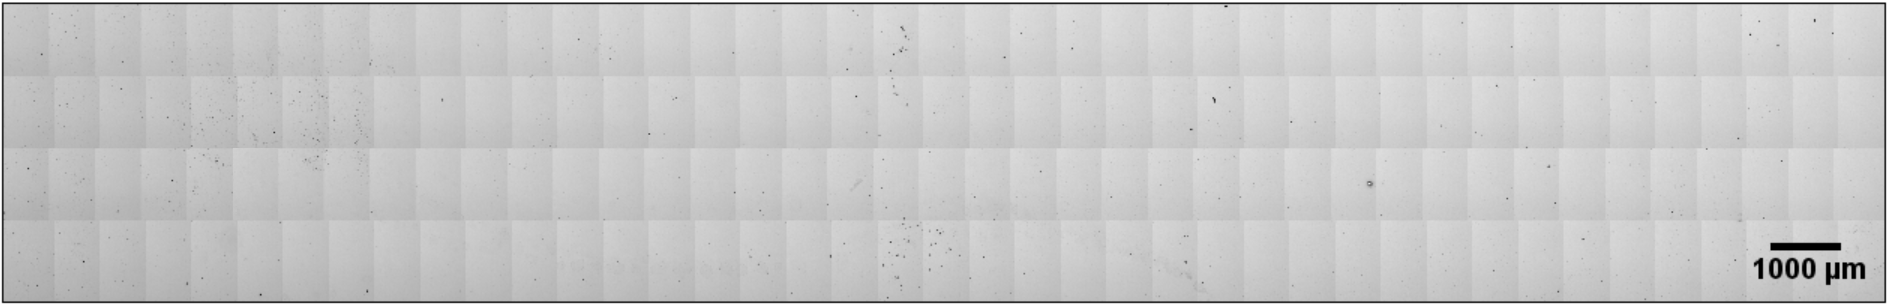
\includegraphics[width=1.0\textwidth]{Figs/cuantificaciondefectos/banda_AZUL.png}
	\caption{Imagen de la banda azul del filtro obtenida mediante un \textit{Tile scan} de 26.37 mm x 4.16 mm, compuesta por 164 \textit{tiles}, con la intensidad de la lámpara configurada en 30\% y el tiempo de exposición de la cámara fue de 40 ms.}
	\label{fig:tilebandaazul}
\end{figure}
\begin{figure}[H]
	\centering
	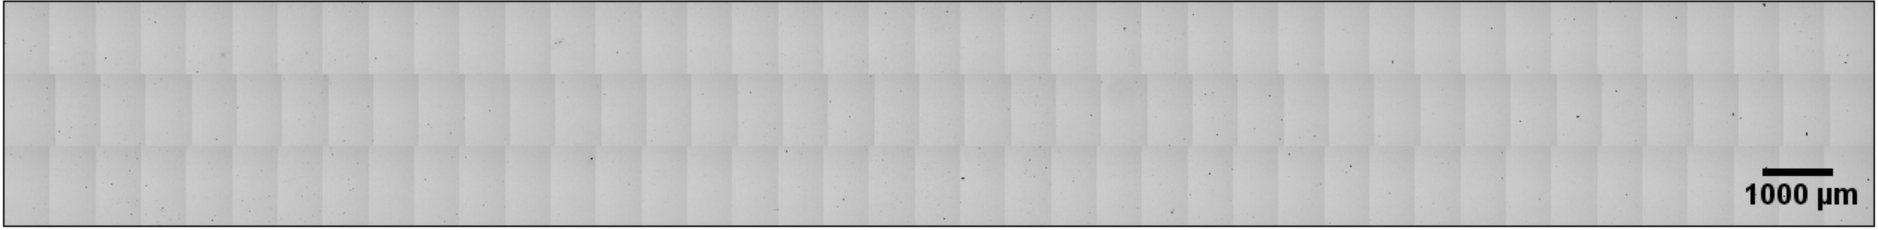
\includegraphics[width=1.0\textwidth]{Figs/cuantificaciondefectos/banda_VERDE.png}
	\caption{Imagen de la banda verde del filtro obtenida mediante un \textit{Tile scan} de 26.37 mm x 3.15 mm, compuesta por 123 \textit{tiles}, con la intensidad de la lámpara configurada en 17\% y el tiempo de exposición de la cámara fue de 40 ms.}
	\label{fig:tilebandaverde}
\end{figure}
\begin{figure}[H]
	\centering
	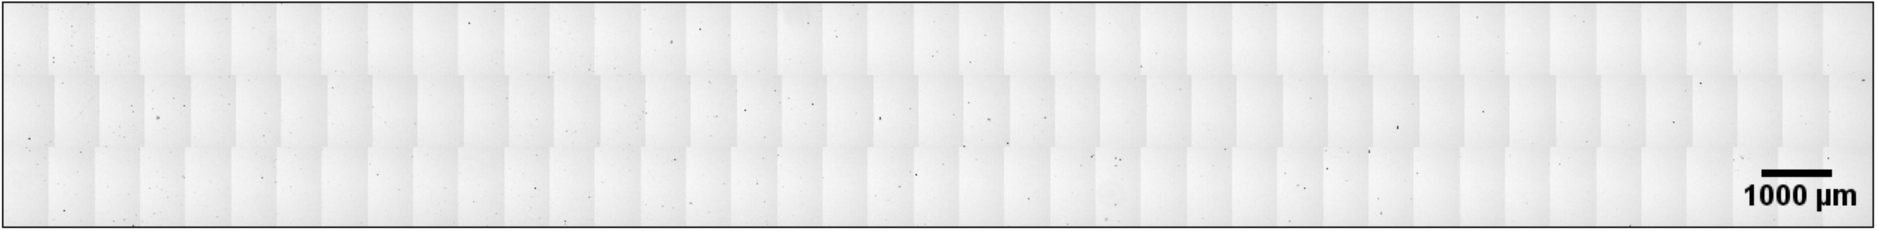
\includegraphics[width=1.0\textwidth]{Figs/cuantificaciondefectos/banda_PANC.png}
	\caption{Imagen de la banda roja del filtro obtenida mediante un \textit{Tile scan} de 26.37 mm x 3.15 mm, compuesta por 123 \textit{tiles}, con la intensidad de la lámpara configurada en 10\% y el tiempo de exposición de la cámara fue de 40 ms.}
	\label{fig:tilebandapanc}
\end{figure}
\begin{figure}[H]
	\centering
	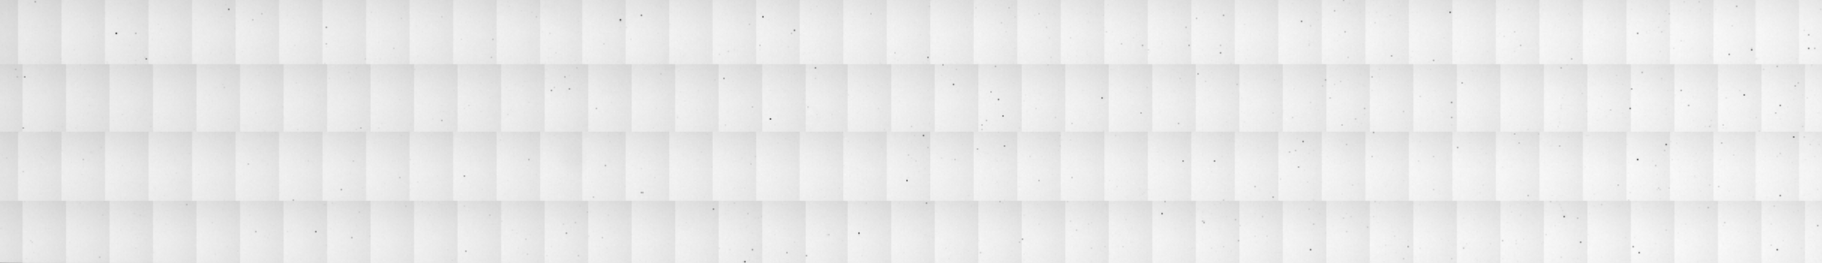
\includegraphics[width=1.0\textwidth]{Figs/defectosZEISS/tilebandaroja.png}
	\caption{Imagen de la banda pancromática del filtro obtenida mediante un \textit{Tile scan} de 27.65 mm x 4.16 mm, compuesta por 124 \textit{tiles}, con la intensidad de la lámpara configurada en 27\% y el tiempo de exposición de la cámara fue de 15 ms.}
	\label{fig:tilebandaroja}
\end{figure}

\begin{figure}[H]
	\centering
	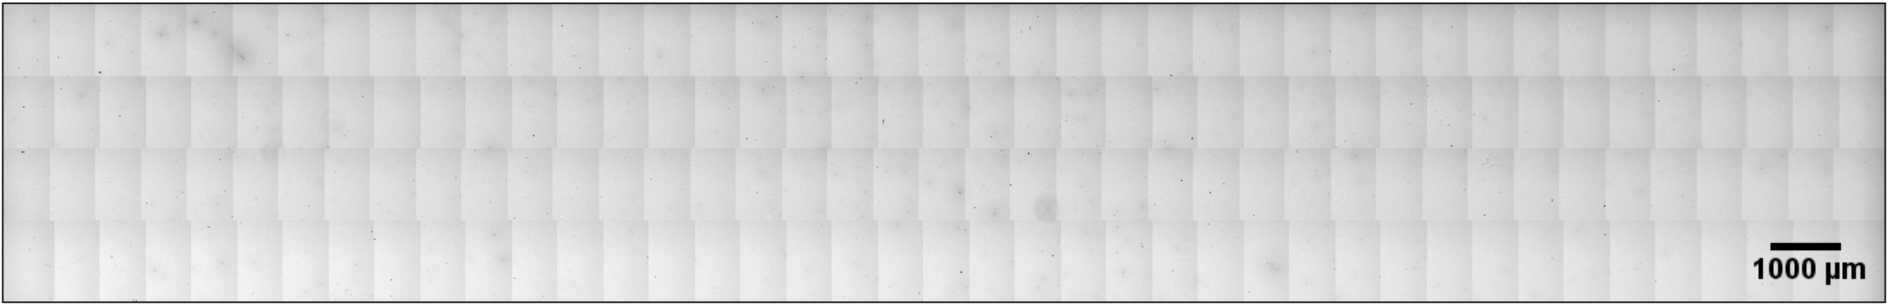
\includegraphics[width=1.0\textwidth]{Figs/cuantificaciondefectos/banda_NIR.png}
	\caption{Imagen de la banda NIR del filtro obtenida mediante un \textit{Tile scan} de 26.37 mm x 4.16 mm, compuesta por 164 \textit{tiles}, con la intensidad de la lámpara configurada en 50\% y el tiempo de exposición de la cámara fue de 150 ms.}
	\label{fig:tilebandanir}
\end{figure}


A continuación se explican algunas consideraciones importantes que se tuvieron respecto de los formatos de las imágenes y de los tipos de datos así como su precisión:
\begin{itemize}
\justifying
\item Cada barrido completo de una banda es guardado por el software de Zeiss en un archivo de extensión .czi que contiene toda la \textit{metadata} como la información referida a la configuración del microscopio utilizada. Dicho archivo puede ser manipulado con el software de Zeiss, ó con el \href{https://imagej.net/Fiji}{Fiji-ImageJ} (tiene más herramientas que el software ImageJ a secas) ó a través del lenguaje \textit{python} utilizando la librería \href{https://pypi.org/project/czifile/}{\textit{czifile}} (Ejemplo sencillo: \href{https://github.com/jrr1984/defects_analysis/blob/master/zeiss_cfi.ipynb}{\faGithub}).
\item El archivo .czi de la banda completa además contiene todas las \textit{tiles} del barrido que pueden ser exportadas como archivos individuales utilizando las herramientas de procesamiento del software de Zeiss \cite{tilezeiss}. Es muy importante exportar dichas imágenes eligiendo un formato de imagen que no modifique la calidad de la imagen original, esto es, que no se pierda precisión sobre los valores de intensidad de cada píxel. 
\item Se recomienda para el guardado, manipulación, operaciones, etc., utilizar el formato de imagen TIFF (\textit{Tagged Image File Format}) pues es un formato que guarda los datos de intensidad de cada píxel originales, sin pérdida de precisión por compresión. Y, definitivamente no se puede utilizar el formato de imagen JPEG (\textit{Joint Photographic Experts Group}) en el campo de la microscopía pues el tipo de compresión que realiza sobre los datos originales resulta en una pérdida de precisión.
\item Por último, se hace notar que la pérdida de precisión de una imagen puede ocurrir tanto en el guardado como en las operaciones sobre las imágenes. Un ejemplo de esta pérdida de precisión sería convertir las imágenes de una precisión original de 16 bits ($2^{16} = 65536$ posibles valores de intensidad) a una precisión de 8 bits ($2^{8} = 256$). Este inconveniente podría ser producido automáticamente por ejemplo en alguna operación utilizando la librería \textit{scikit-image} \cite{van2014scikit}, por lo que se sugiere controlar la precisión con la que se manipulan las imágenes en cada operación realizada.
\end{itemize}

La eficiencia en la aplicación de un algoritmo de segmentación\footnote{En el contexto de la presente tesis, el término segmentación hace referencia a la identificación individual de cada defecto presente en una imagen.} de defectos en las imágenes individuales de cada banda adquiridas depende fuertemente de la distribución de los valores de intensidad de una imagen que permiten distinguir a los defectos del fondo de la imagen. A continuación se da una breve explicación sobre las consecuencias de una iluminación no uniforme del microscopio sobre una muestra y como esto repercute en la detección posterior de los defectos. Luego se explica el procesamiento de las imágenes realizado para obtener la cuantificación de los defectos de cada banda del filtro.

\singlespacing
\section{Iluminación no uniforme del microscopio}
\label{sec:ilumnou}
\spacing{1.5}

\hspace{0.5cm}Las imágenes microscópicas pueden estar corrompidas por las variaciones de intensidad debido a las imperfecciones inherentes del proceso de formación de imágenes. Estas variaciones de intensidad pueden venir dadas por la iluminación no uniforme de la muestra, por la orientación misma de la muestra al montarla sobre la platina del microscopio ó por el efecto de \textit{vignetting} (la aparición de bordes negros en las imágenes) propio de la configuración del sensor de la cámara. Estos efectos pueden dar lugar a falsos positivos\footnote{En el contexto de esta tesis, un falso positivo consistiría en la detección errónea mediante un algoritmo de procesamiento de imágenes de un defecto que en realidad no lo es.} en el proceso de segmentación de los defectos, lo que constituye un grave problema a solucionar.

La desalineación de alguno de los componentes que se encuentran en el camino óptico entre la fuente de luz y el sensor de la cámara con el que se adquieren las imágenes (Ver Figura \ref{fig:micczeiss}), es una causa muy importante de la iluminación no uniforme de la muestra que se está analizando. En la Figura \ref{fig:ejnounif} se puede observar un ejemplo de una imagen micróscopica adquirida con una iluminación no uniforme.
	\begin{figure}[H]
		\begin{floatrow}
			\ffigbox{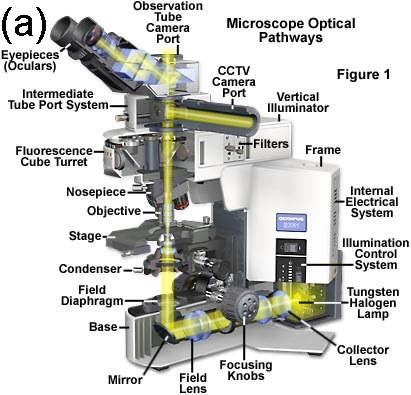
\includegraphics[scale=0.5]{Figs/defectosZEISS/opticalpaths.jpg}}{\caption{Camino óptico de la luz desde su fuente de emisión hasta la detección en el sensor de una cámara digital. Adaptado de \href{https://bit.ly/2xrh8Jh}{https://bit.ly/2xrh8Jh}}\label{fig:micczeiss}}
			\ffigbox{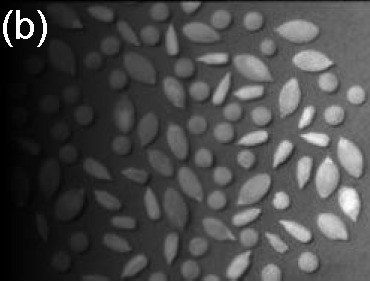
\includegraphics[scale=0.5]{Figs/cuantificaciondefectos/ilumnoun.png}}{\caption{Ejemplo de imagen microscópica con una iluminación no uniforme.}\label{fig:ejnounif}}
		\end{floatrow}
	\end{figure}
	
Una imagen microscópica adquirida idealmente con una iluminación uniforme perfecta tendría una imagen de fondo (\textit{background image}) como la que se muestra en la Figura \ref{fig:fondideal}. La imagen de fondo es una imagen que contiene en cada píxel la información de la iluminación del microscopio bajo ciertas condiciones de intensidad de la fuente de luz y del tiempo de integración del sensor de la cámara utilizado. Experimentalmente, dicha imagen puede ser obtenida colocando un portaobjeto sin la muestra, en las mismas condiciones de iluminación y foco (misma distancia muestra-objetivo). Si dicha imagen de fondo experimental no pudiera ser adquirida pero se cuenta con un gran número de imágenes bajo las mismas condiciones experimentales, una imagen de fondo puede ser generada tomando la mediana del conjunto de imágenes como se explica más adelante.

Para medir la uniformidad de la iluminación se utilizan los histogramas de las imágenes. Una imagen monocromática es manipulada computacionalmente como una matriz donde cada elemento de la matriz representa el valor de intensidad de dicho píxel asociado. El histograma de una imagen es la representación de la distribución de intensidad de la misma y se lo define como el número de píxeles presentes en una imagen con un cierto valor de intensidad.

En la Figura \ref{fig:fondideal} se muestra una imagen de fondo ficticia que tendría una iluminación ideal uniforme y sin problemas de  \textit{vignetting}. Dicha imagen tiene un histograma como el que se muestra en la Figura \ref{fig:histbgteo}, en el que se puede observar que todos los píxeles de la imagen tienen el mismo valor de intensidad, lo que demuestra que el fondo es perfectamente homogéneo.
	\begin{figure}[H]
		\begin{floatrow}
			\ffigbox{
\includegraphics[width=5.0cm,height=6.0cm]{Figs/defectosZEISS/bg_teorico.png}}{\caption{Imagen de fondo con una iluminación uniforme ideal y sin problemas de \textit{vignetting}. }\label{fig:fondideal}}
			\ffigbox{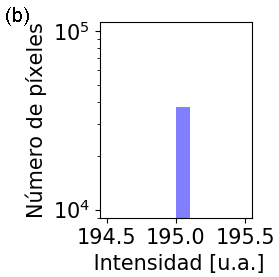
\includegraphics[scale=1.3]{Figs/defectosZEISS/hist_bg_teorico.png}}{\caption{Histograma de la intensidad de los píxeles de la imagen de fondo ideal.}\label{fig:histbgteo}}
		\end{floatrow}
	\end{figure}
En adelante, el fondo de cada imagen será denominado el \textit{background} de la imagen, para diferenciarlo de los defectos que se encuentran en lo que en adelante se llamará el \textit{foreground} de la imagen. Para resaltar la importancia de la corrección de la iluminación no uniforme y del \textit{vignetting}, supongamos una imagen ficticia de alguna banda del filtro analizado en la presente tesis, adquirida con una iluminación de fondo uniforme ideal y sin problemas de \textit{vignetting}, donde se puedan observar dos defectos (en color negro).
	\begin{figure}[H]
		\begin{floatrow}
			\ffigbox{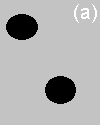
\includegraphics[width=5.0cm,height=7.0cm]{Figs/defectosZEISS/img_ideal_2defectos.png}}{\caption{Imagen con dos defectos con una iluminación uniforme ideal y sin problemas de \textit{vignetting}. }\label{fig:ideal2def}}
			\ffigbox{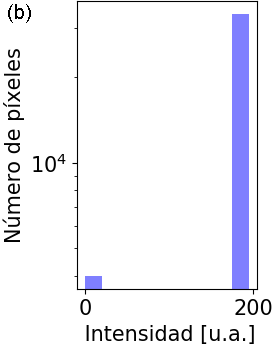
\includegraphics[scale=1.2]{Figs/defectosZEISS/hist_bg_condefectos_teorico.png}}{\caption{Histograma de la intensidad de los píxeles de la imagen con dos defectos con una iluminación uniforme ideal y sin problemas de \textit{vignetting}.}\label{fig:histideal2def}}
		\end{floatrow}
	\end{figure}
En la Figura \ref{fig:histideal2def} se muestra el histograma de la intensidad de los píxeles de la imagen con dos defectos con una iluminación uniforme ideal y sin problemas de \textit{vignetting}. En dicho histograma se distingue de forma binaria el \textit{foreground} (defectos) con valores de intensidad iguales a 0, del \textit{background} con valores de intensidad iguales a 195. Bajo estas condiciones ideales, la segmentación de los defectos puede ser realizada de inmediato eligiendo cualquier umbral de intensidad que se encuentre entre el \textit{foreground} y el \textit{background}. 

A continuación se explica el análisis computacional de las imágenes individuales de cada banda realizado desde su pre-procesamiento, la segmentación posterior y finalmente la cuantificación de los defectos.

\singlespacing
\section{Pre-pocesamiento de las imágenes de cada banda espectral }
\spacing{1.5}

\hspace{0.5cm}El análisis de las imágenes fue realizado sobre cada \textit{tile} individual del barrido completo de una banda, dado que su tamaño típico es de 3 MB por lo que el procesamiento en la computadora es mucho más rápido que el de analizar las imágenes de una banda completa\footnote{Vale aclarar que las imágenes completas ya sea de una banda ó las del filtro completo, fueron el resultado de realizar un \textit{stitching} de todas las \textit{tiles} individuales de cada adquisición y, fueron procesadas de esta manera simplemente para optimizar su visualización pero no para realizar el análisis ni detección de defectos sobre las mismas.}, de tamaños típicos de 1 GB ó del filtro completo que tienen más de 5 GB.

El pre-procesamiento de las imágenes individuales de cada banda espectral consistió en la corrección de la iluminación no uniforme del microscopio que se realiza normalizando las imágenes individuales del barrido con una imagen de fondo \cite{Nordenfelt}. Este pre-procesamiento consistió de las siguientes dos etapas que se explican a continuación:
\begin{enumerate}
\justifying
\item Generación de la imagen de fondo.
\item Normalización de las imágenes individuales del barrido de una banda con la imagen de fondo.
\end{enumerate}

\singlespacing
\subsection{Generación de la imagen de fondo: \href{https://github.com/jrr1984/defects_analysis/blob/master/MAIN/bg.py}{\faGithub}}
\spacing{1.5}

\hspace{0.5cm}Se construyó computacionalmente la imagen de fondo de cada banda a partir de tomar la \underline{mediana} para cada píxel de todas las imágenes individuales adquiridas de la banda. Esta imagen de fondo contiene la información de la no uniformidad de la iluminación del microscopio. Dicha imagen debe ser generada para cada banda en particular ya que cada una de las bandas fue adquirida en ciertas condiciones de intensidad de la fuente de luz y del tiempo de integración de la cámara. 

En la Figura \ref{fig:bgazul} se muestra la imagen de fondo generada para la banda azul, cuya intensidad de la fuente de luz fue configurada en 30$\%$ y el tiempo de integración de la cámara fue de 40 ms. Los dos discos concéntricos que se observan en la imagen son resultado de alguna reflexión no deseada en el microscopio, ya advertida por otros usuarios del equipo. Dichos discos fueron observados en la adquisición de las cinco bandas. 
	\begin{figure}[H]
		\begin{floatrow}
			\ffigbox{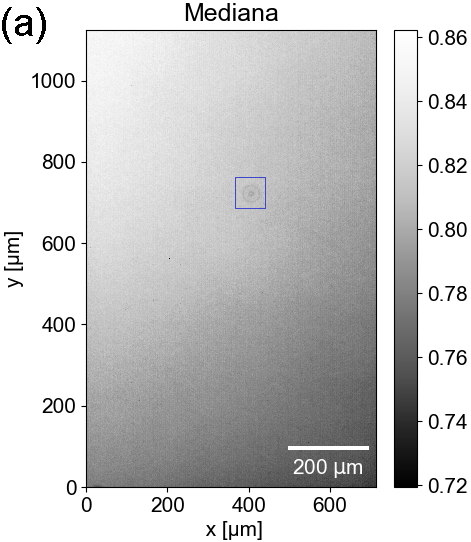
\includegraphics[scale=0.9]{Figs/defectosZEISS/bg_azul.png}}{\caption{Imagen de fondo de la banda azul del filtro obtenida tomando la \underline{mediana} para cada píxel de todas las imágenes del barrido.}\label{fig:bgazul}}
			\ffigbox{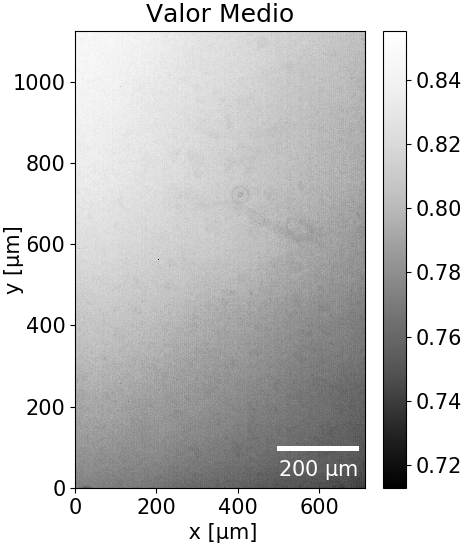
\includegraphics[scale=0.9]{Figs/defectosZEISS/bg_azul_mean.png}}{\caption{Imagen de fondo de la banda azul del filtro obtenida tomando el \underline{valor medio} para cada píxel de todas las imágenes del barrido.}\label{fig:bgazulmean}}
		\end{floatrow}
	\end{figure}
Al mismo tiempo, se observa en la imagen de fondo de la Figura \ref{fig:bgazul} que la iluminación del microscopio no es idealmente uniforme sino que presenta un rango de valores de intensidad que contienen píxeles más brillantes (extremo superior izquierdo) en conjunto con píxeles más oscuros (extremo inferior derecho). Esto último puede ser el efecto de alguna desalineación de la configuración del microscopio.

En la Figura \ref{fig:comparhists} se muestran los histogramas de la intensidad de los píxeles de las imágenes de fondo generadas a partir de tomar la mediana y el valor medio. En la misma figura se graficaron las curvas de densidad estimadas a partir de los datos originales. Se observa que la imagen de fondo generada con el valor medio tiene una mayor cantidad de píxeles más oscuros que la imagen de fondo generada con la mediana. Los valores atípicos (en inglés \textit{outliers}) de intensidad influencian enormemente el valor medio de los datos. Dichos \textit{outliers} pueden observarse como manchas presentes en la imagen de fondo generada a partir del valor medio de la Figura \ref{fig:bgazulmean} y en la curva de densidad esto se refleja en el hecho de que la curva del valor medio tiene una mayor concentración en valores de intensidades más chicos que la curva de la mediana. Ahora bien, la curva de densidad de la imagen de la mediana muestra que la generación de la imagen de fondo tomando la mediana es una forma exitosa de evitar incluir los \textit{outliers} en la imagen. Resulta fundamental deshacerse de estos \textit{outliers} en la imagen de fondo para no corromper las imágenes individuales originales del barrido. Esto es, si se utilizara la imagen de fondo del valor medio para corregir la iluminación no uniforme en las imágenes individuales, las mismas tendrían luego los \textit{outliers} presentes lo cual sería catástrofico.
\begin{figure}[H]
	\centering
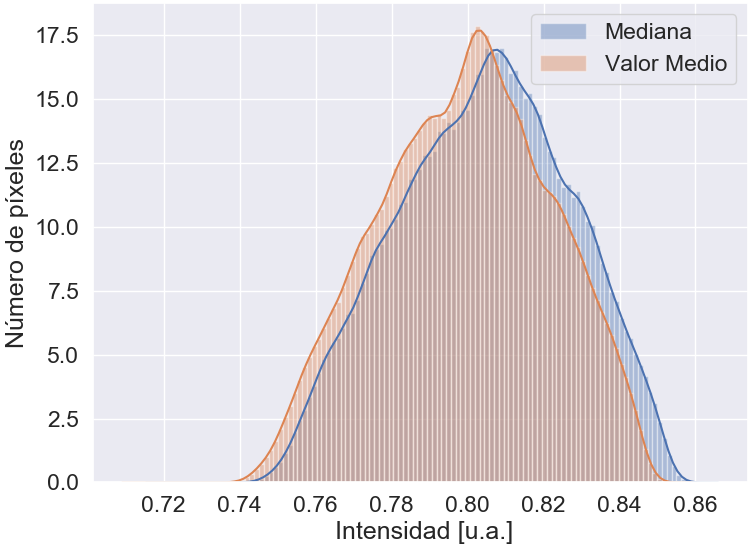
\includegraphics[scale=0.9]{Figs/defectosZEISS/comparhistsmedi.png}
\caption{Histogramas de las imágenes de fondo de la banda azul del filtro generadas a partir de tomar el valor medio y la mediana para cada píxel del conjunto de imágenes de la banda. Se graficaron simultáneamente las curvas de distribución estiamdas a partir de los datos de las imágenes. El eje vertical se encuentra normalizado por el máximo valor de la frecuencia de píxeles para un cierto valor de intensidad.}
\label{fig:comparhists}
\end{figure}	
Se hace notar por un lado que para generar la imagen de fondo se utiizaron las imágenes originales de cada banda y que al ser manipuladas en el lenguaje de programación \textit{python} para tomarles la mediana, dichas imágenes fueron tratadas como matrices donde cada elemento de matriz contenía un valor numérico cuyo tipo de dato computacional era un entero sin signo de 16 bits de precisión, es decir un número entre 0 y 65536. Dichos valores son tratados como números de punto flotante, con una precisión de 64 bits al momento de tomar la mediana para cada píxel del conjunto de imágenes. En consecuencia la imagen de salida tiene la misma precisión y los valores de intensidad son reescaleados al intervalo comprendido entre 0 y 1.

A continuación se explica el proceso de corrección de la iluminación no uniforme del microscopio en las imágenes individuales de cada banda adquirida.	
	
\singlespacing
\subsection{Normalización de las imágenes individuales del barrido de una banda con la imagen de fondo \href{https://github.com/jrr1984/defects_analysis/blob/master/MAIN/bg_normalization.py}{\faGithub}}
\spacing{1.5}

\hspace{0.5cm} Con la imagen de fondo de cada banda ya construida, se normalizaron las imágenes originales del barrido completo de cada banda\cite{Nordenfelt} con el objetivo de corregir la iluminación no uniforme del microscopio y para eliminar la reflexión no deseada del objetivo del microscopio presente en todas las imágenes (discos concéntricos de la imagen \texttt{b)} de la Figura \ref{fig:bgazul}).
\begin{figure}[H]
	\centering
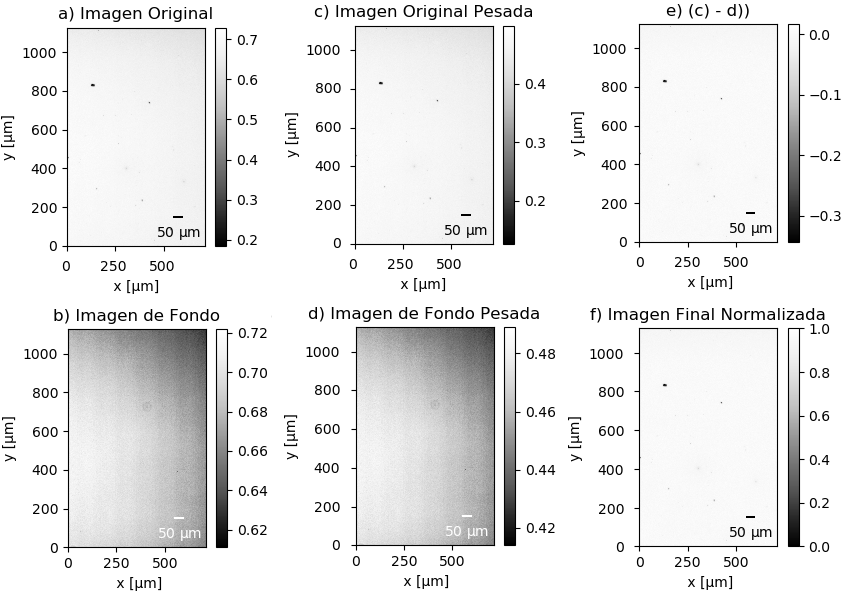
\includegraphics[scale=0.98]{Figs/defectosZEISS/correccionilum/NIR/1.png}
\caption{Imágenes del proceso de corrección de la iluminación no uniforme. \texttt{a)} Imagen original individual de la banda NIR.\texttt{b)} Imagen de fondo de la banda NIR. \texttt{c)} Imagen original multiplicada por el valor medio de la imagen de fondo. \texttt{d)} Imagen de fondo multiplicada por el valor medio de la imagen original. \texttt{e)} Imagen resultante de la diferencia entre las imágenes \texttt{c)} y \texttt{d)}. \texttt{e)} Imagen final normalizada resultado de la expansión del histograma de intensidades.}
\label{fig:correcilumims}
\end{figure}	
 En la Figura \ref{fig:correcilumims} se muestran las operaciones del proceso de normalización de una imagen individual (\textit{tile}) del barrido completo de la banda NIR. El mismo proceso fue realizado para cada imagen individual de cada banda adquirida de acuerdo a las siguientes operaciones:
\begin{itemize}
\justifying
\item Se calculó el valor medio de la intensidad de la imagen de fondo (\textit{bg\_img}, ver imagen \texttt{b)}) y de la imagen individual (\textit{tile\_img}, ver imagen \texttt{a)}) de una banda a normalizar. Esto es, se calculó la media aritmética de todos los elementos de matriz que representan a cada imagen, que es el resultado de la división entre la suma de todos los elementos de la matriz y el número total de los mismos.
\item Se multiplicó la imagen de fondo por el valor medio de la imagen individual y viceversa, es decir:
\begin{equation}
\textit{bg\_pes} = mean(\textit{tile\_img})\hspace{2pt} . \hspace{2pt}\textit{bg\_img}
\end{equation}
\begin{equation}
\textit{tile\_pes} = mean(\textit{bg\_img})\hspace{2pt} . \hspace{2pt}\textit{tile\_img}
\end{equation},
donde \textit{bg\_pes} (Ver imagen \texttt{d)}) y \textit{tile\_pes} (Ver imagen \texttt{c)}) son la imagen de fondo y la imagen individual pesadas con la contribución del valor medio de la imagen correspondiente.
\item Se corrigió la iluminación no uniforme de la imagen original (Ver imagen \texttt{e)}), cuya imagen resultante se la denomia \textit{dif}:
\begin{equation}
\textit{dif} = \textit{tile\_pes} - \textit{bg\_pes}
\end{equation}
\item Finalmente, para maximizar el contraste de la imagen, es decir para aumentar la variación de los valores de intensidad de la imagen, se realizó la expansión del histograma (\cite{anilfund}) que consiste en una transformación lineal para expandir el intervalo comprendido entre los valores mínimo y máximo de intensidad presentes en la imagen, a todo el rango posible entre 0 y 1 (Ver Ecuación \ref{eq:histexpp}). Para ello, se definió el mínimo valor de la intensidad en 0 (en un rango de valores de intensidad entre 0 y 1, con precisión de 64 bits):
\begin{equation}
	\textit{min\_dif} = \textit{dif} - min(\textit{dif})
\end{equation},
donde min(\textit{dif}) es el mínimo valor de intensidad de la imagen \textit{dif}. A la imagen resultante \textit{min\_dif} se la normaliza de la siguiente manera:
\begin{equation}
	\textit{imagen\_final} = \frac{\textit{min\_dif}}{max(\textit{dif})-min(\textit{dif})} = \frac{\textit{dif} - min(\textit{dif})}{max(\textit{dif})-min(\textit{dif})}
	\label{eq:histexpp}
\end{equation},
donde max(\textit{dif}) es el máximo valor de intensidad de la imagen \textit{dif} e \textit{imagen\_final} es la imagen resultante del proceso de normalización.
\end{itemize}

Se hace notar que el proceso de corrección de la iluminación no uniforme y del \textit{vignetting} resultó fundamental para poder aplicar el algoritmo de detección de los defectos, esto es para distinguir el \textit{foreground} del \textit{background}, como se explicó en la sección \ref{sec:ilumnou}. Para ejemplificar esto y para ilustrar la operación de la expansión del histograma de la ecuación \ref{eq:histexpp}, en la Figura \ref{fig:defecthi} se muestra una región con un defecto de la imagen original y de la final así como los histogramas de intensidad de los píxeles de la diagonal de la misma región asociados.


\begin{figure}[H]
	\centering
	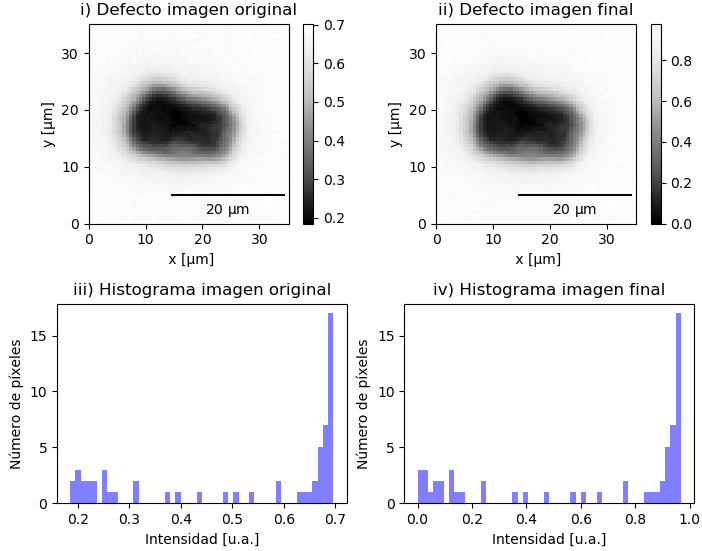
\includegraphics[scale=1.0]{Figs/defectosZEISS/correccionilum/defectoehist.png}
	\caption{\texttt{i)} Imagen original de una región con un defecto. \texttt{ii)} Imagen resultante del proceso de normalización de la misma región que \texttt{i)}. \texttt{iii)} Histograma de los píxeles de la diagonal de la imagen \texttt{i)}. \texttt{iv)} Histograma de los píxeles de la diagonal de la imagen \texttt{ii)}.}
	\label{fig:defecthi}
\end{figure}

De la comparación entre los histogramas \texttt{iii)} y \texttt{iv)} se observa que el rango de intensidades de los píxeles de la región con un defecto de la imagen original se extiende desde el intervalo [0.19,0.70] al intervalo [0.00,0.98] en la imagen final\footnote{Para la imagen completa, el rango se extiende desde [0.19,0.73] para la imagen original al rango [0.00,1.00] de la imagen final, es decir el rango de intensidades de la imagen original se extiende a todo el rango posible de acuerdo a la ecuación \ref{eq:histexpp} de la expansión del histograma.}. De esta manera, se mejora el contraste de la imagen y la distinción entre el \textit{foreground} (defectos) y el \textit{background} se puede realizar ajustando un umbral de intensidad  (\textit{threshold}). A continuación se explica el criterio de elección del método del \textit{threshold} aplicado y luego se describe el algoritmo de detección de los defectos y su cuantificación.

\singlespacing
\section{Criterio de elección del \textit{threshold} \href{https://github.com/jrr1984/defects_analysis/blob/master/MAIN/try_all_thresholds.py}{\faGithub}}
\spacing{1.5}

\hspace{0.5cm}Con las imágenes pre-procesadas la detección de los defectos fue realizada utilizando algoritmos de procesamientos de imágenes. En particular se utilizaron algoritmos de \textit{thresholding} que determinan un umbral de intensidad a partir del cual se crea una imagen binaria que distingue el \textit{background} de los defectos \cite{shapi}.

Para determinar el umbral de intensidad óptimo para todas y cada una de las imágenes individuales de una banda se utilizó el método \textit{try\_all\_threshold} de la librería \textit{scikit-image} del lenguaje \textit{python} \cite{van2014scikit}. Se hace notar que si bien se podrían haber utilizado distintos \textit{thresholds} para cada imagen ó para distintos sets de imágenes de una misma banda, se decidió elegir un sólo método de umbral para todas y cada una de las bandas para poder automatizar la aplicación del algoritmo de detección de los defectos y de la posterior asociación de incertezas a los resultados.

El criterio de elección del método del umbral fue adoptado a partir de la inspección visual. Se observó visualmente el resultado (en adelante \textit{output}) de la aplicación de los distintos \textit{thresholds} para cada imagen de cada banda. A continuación se muestran algunas imágenes representativas en conjunto con el \textit{output} de la aplicación de los distintos \textit{thresholds} para explicar el criterio de elección del umbral aplicado a todas las imágenes de todas las bandas.
\begin{enumerate}
\justifying
\item Se descartaron los \textit{thresholds} a partir de los cuales algunas de las imágenes binarias generadas contenían una gran cantidad de falsos positivos. Esto último resultó ser el caso de los métodos \textit{Li}\cite{Lie}, \textit{Mean}\cite{Glasmean} y \textit{Otsu}\cite{otsuu}, como se puede observar en la Figura \ref{fig:threshcom}. Por el motivo contrario, es decir por no contener ningún defecto en algunas de las imágenes binarias generadas, el umbral \textit{Minimum}\cite{pericles} fue descartado.
\begin{figure}[H]
	\centering
	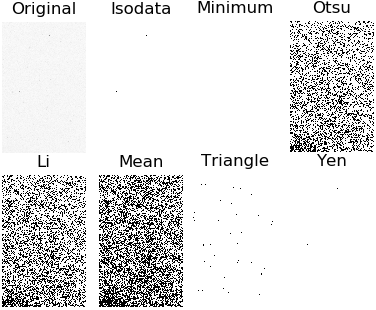
\includegraphics[scale=2.3]{Figs/defectosZEISS/thresh_comparison.png}
	\caption{Figura del \textit{output} del método \textit{try\_all\_threshold} de la librería \textit{scikit-image} del lenguaje \textit{python} (Ver \href{https://github.com/jrr1984/defects_analysis/blob/master/MAIN/try_all_thresholds.py}{\faGithub}).} 
	\label{fig:threshcom}
\end{figure}

\item Si bien en la gran mayoría de las imágenes los métodos \textit{Isodata}\cite{ridler}, \textit{Triangle}\cite{triang} y \textit{Yen}\cite{yen} tuvieron una buena relación entre el número de falsos positivos y el número de defectos detectados por inspección visual, el único \textit{threshold} que mantuvo dicha relación con un valor menor a 1 para todas las imágenes de todas las bandas fue el del método \textit{Yen}. Por ejemplo en la Figura \ref{fig:threshcom2} se muestra una región de una imagen con 2 defectos detectados por inspección visual y el método \textit{Yen} fue el único capaz de detectarlos de forma singular.

\begin{figure}[H]
	\centering
	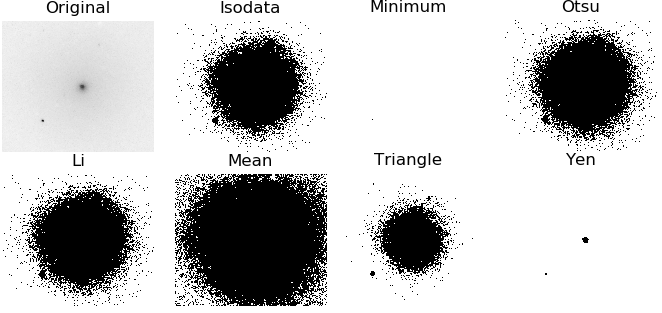
\includegraphics[scale=1.2]{Figs/defectosZEISS/thresh_vivos_compar3.png}
	\caption{Región de una imagen individual en conjunto con el \textit{output} de lFigura del \textit{output} del método \textit{try\_all\_threshold} de la librería \textit{scikit-image} del lenguaje \textit{python} (Ver \href{https://github.com/jrr1984/defects_analysis/blob/master/MAIN/try_all_thresholds.py}{\faGithub}).} 
	\label{fig:threshcom2}
\end{figure}
%# de defectos por metodo: yen,isodata,triangle
%2828,4439,274176  ROJO
%4015,6674,156695 PANC
%5727,11010,234359 VERDE
%19918,40505, AZUL
\end{enumerate}
\hspace{0.5cm}Una vez determinado el \textit{threshold} aplicable a todas las imágenes de todas las bandas, se desarrolló el algoritmo de detección y cuantificación de los defectos del filtro que se explica en la siguiente sección.

\singlespacing
\section{Algoritmo de detección y cuantificación de los defectos \href{https://github.com/jrr1984/defects_analysis/blob/master/MAIN/defects_thresholding.py}{\faGithub}}
\label{sec:secalg}
\spacing{1.5}

\hspace{0.5cm}En esta sección se explica el algoritmo utilizado para la detección y cuantificación de los defectos del filtro. El diagrama de flujo del algoritmo aplicado se muestra en la Figura \ref{fig:diagflujoalgor}. 

\begin{figure}[H]
\centering
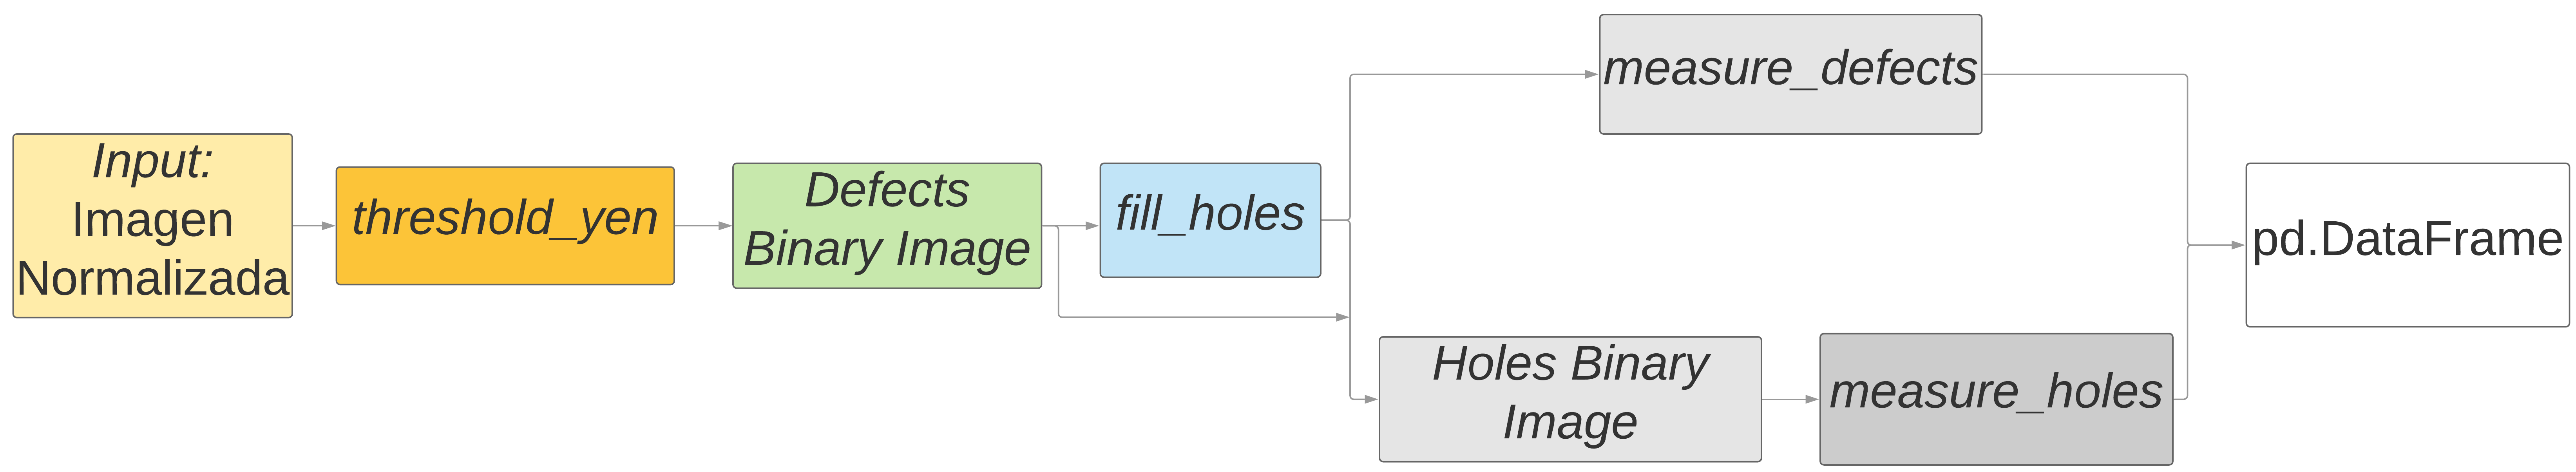
\includegraphics[scale=0.8]{Figs/cuantificaciondefectos/diag_flujoalgor.png}
\caption{Diagrama de flujo del algoritmo de detección y cuantificación de los defectos del filtro.}
\label{fig:diagflujoalgor}
\end{figure}


\begin{figure}[H]
\centering
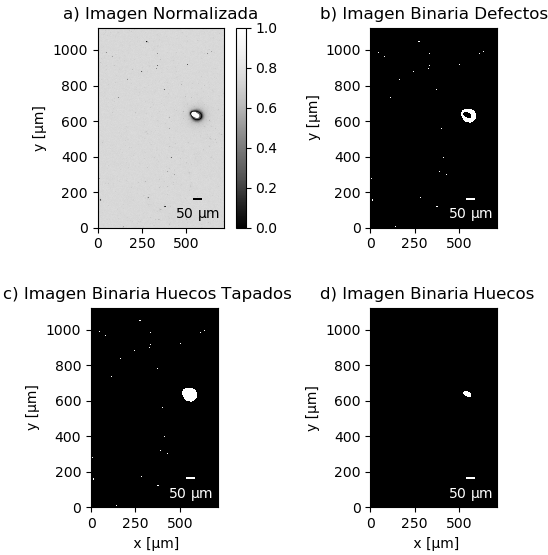
\includegraphics[scale=1.5]{Figs/defectosZEISS/algor_defecs.png}
\caption{\texttt{a)} Imagen normalizada de la banda celeste que contiene un agujero.  \texttt{b)} Imagen binaria generada a partir del \textit{threshold} de \textit{Yen}. \texttt{c)} Imagen con los agujeros de la imagen \texttt{b)} tapados con el método \textit{binary\_fill\_holes} de la clase \textit{ndimage} de la librería \textit{scipy} del lenguaje \textit{python}. \texttt{d)} Imagen binaria con el agujero detectado.}
\label{fig:flujoalgo}
\end{figure} 

Utilizando el diagrama de flujo de la Figura \ref{fig:diagflujoalgor} y la Figura \ref{fig:flujoalgo} como guías didácticas, a continuación se explican los pasos del algoritmo aplicado para cada imagen individual de cada banda:
\begin{enumerate}
\justifying
\item \texttt{INPUT: Imagen Normalizada.} Se lee la imagen normalizada. En la imagen \texttt{a)} de la Figura \ref{fig:flujoalgo} se muestra una imagen normalizada de la banda azul que contiene el agujero más grande encontrado en el filtro (caracterizado espectralmente en el Capítulo \ref{chap:microsp}) y otros defectos de transmisión (manchas negras) más pequeños. En consecuencia, la imagen es representativa de lo que sería el caso más general de la aplicación del algoritmo para detectar tanto defectos de transmisión como agujeros. 
\item \texttt{\textit{threshold\_yen}.} Se calcula el \textit{threshold} de \textit{Yen} con el método \textit{threshold\_yen} de la librería \textit{scikit-image}. En la Figura \ref{fig:histalgor} se muestra el histograma de intensidad de píxeles de la imagen, con el eje vertical en escala logarítmica. La línea vertical roja indica el valor calculado del \textit{threshold} de \textit{Yen} que para esta imagen de ejemplo su valor fue de 0.57. Se hace notar que dicho valor de intensidad umbral es global de toda la imagen y para cada imagen se calcula un \textit{threshold} de \textit{Yen} individual.

\begin{figure}[H]
\centering
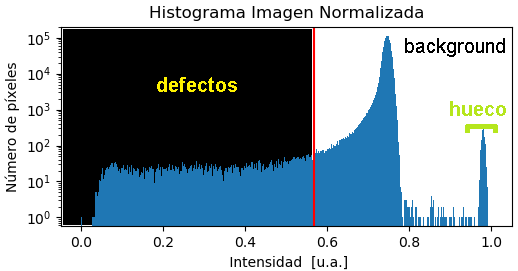
\includegraphics[scale=1.65]{Figs/defectosZEISS/hist_algor_agujero.png}
\caption{Histograma de intensidad de los píxeles de la imagen \texttt{a)} de la Figura \ref{fig:flujoalgo}, con el eje vertical en escala logarítmica. La línea roja vertical indica el valor del \textit{threshold} de \textit{Yen} para dicha imagen.}
\label{fig:histalgor}
\end{figure}

\item \texttt{Defects Binary Image.}Se genera una imagen binaria de la imagen normalizada como se muestra en la imagen \texttt{c)} de la Figura \ref{fig:flujoalgo}. Para cada píxel de la imagen normalizada se compara su valor de intensidad con el valor del \textit{threshold} y se asigna un 1 (blanco, \textit{background} y agujeros) si el valor de intensidad del píxel es mayor que el \textit{threshold} y un 0 (negro, defectos) si ocurre lo contrario. Esto último se puede ver en el histograma de la Figura \ref{fig:histalgor}.
\item \texttt{\textit{fill\_holes}.} Se tapan los agujeros como se muestra en la imagen \texttt{d)} de la Figura \ref{fig:flujoalgo} con el método \textit{binary\_fill\_holes} de la clase \textit{ndimage} de la librería \textit{scipy} del lenguaje \textit{python} \cite{scipy}.

\hspace{0.5cm}Se hace notar que \underline{en el contexto de imágenes binarias} un defecto de transmisión es un objeto matricial de ciertas dimensiones en píxeles cuyos elementos de matriz son \underline{todos} iguales a 1 (color blanco). Y, un agujero es un objeto matricial cuyo borde tiene elementos de matriz iguales a 1 (color blanco) pero los elementos de matriz del interior de dicho borde son iguales a 0 (color negro). Lo que el método \textit{binary\_fill\_holes} realiza es encontrar objetos que cumplan la condición matricial de un agujero y llenar su interior de píxeles blancos. El tamaño del agujero a tapar puede ser elegido por el usuario a partir de las dimensiones de la matriz de píxeles blancos utilizada. Esta matriz es especificada en el argumento \textit{structure} del método \textit{binary\_fill\_holes} y es un parámetro fundamental que debe ser especificado de acuerdo a los requerimientos de calidad óptica del usuario ya que su tamaño define el tamaño mínimo del agujero a detectar. En la presente tesis dicho parámetro fue dejado sin especificar, el método tomó el valor por \textit{default} por lo que todos los agujeros encontrados fueron tapados.

\hspace{0.5cm}A continuación se explica la bifurcación en el algoritmo de la detección de defectos en general por un lado sin discriminar su tipo y la detección específica de agujeros por el otro lado.

\item \texttt{\textit{measure\_defects}}. La detección de los defectos en general fue realizada sobre las imágenes binarias con los agujeros tapados (Ver imagen \texttt{c)} de la Figura \ref{fig:flujoalgo}). En consecuencia, no se distinguieron los agujeros de los defectos de transmisión, sino que todos los defectos fueron considerados defectos de superficie de acuerdo a las especificaciones técnicas de la ISO 10110 (Ver Sección \ref{sec:iso10110}). Por este motivo resultó importante realizar el tapado de los agujeros ya que sino se modificaría el valor del área total de los defectos con estas características, considerando a estos como un solo objeto compuesto por una mancha negra que bordea a un agujero blanco, como por ejemplo de acuerdo al defecto más grande de la Figura \ref{fig:flujoalgo}. Este mismo defecto sin tapar tenía un área (dada por el número de píxeles) de (4108.39 $\pm$ 0.59)$\mu m^{2}$ pero el mismo agujero tapado, es decir el defecto a estimar, tenía un área de (5174.29 $\pm$ 0.59)$\mu m^{2}$, por lo que se hubiese obtenido un 20.6\% de error.

\hspace{0.5cm}En la imagen binaria con los agujeros tapados, los defectos ya se encontraban segmentados, es decir que los defectos eran regiones aisladas de píxeles blancos conectados entre sí. El método \href{https://scikit-image.org/docs/dev/api/skimage.measure.html#skimage.measure.label}{\textit{measure.label}} etiqueta a cada uno de los defectos cuyas propiedades son calculadas con el método \href{https://scikit-image.org/docs/dev/api/skimage.measure.html#skimage.measure.regionprops_table}{\textit{measure.regionprops\_table}} y luego guardadas en un \href{https://pandas.pydata.org/pandas-docs/stable/reference/api/pandas.DataFrame.html}{\textit{DataFrame}} de la librería \textit{pandas}\cite{pandas}\footnote{Un \textit{DataFrame} de \textit{pandas} es una estructura de datos que permite una rápida visualización de los datos como en una planilla de excel y que tiene una gran familia de métodos a su disposición para realizar un análisis cuantitativa de los datos.}. Las propiedades de los defectos calculadas fueron el área y el diámetro equivalente\footnote{Muchas otras propiedades podrían haber sido también calculadas automáticamente pero no fueron necesarias en el presente trabajo (Ver \href{https://github.com/scikit-image/scikit-image/blob/master/skimage/measure/\_regionprops.py\#L643}{\textit{measure.regionprops}}).}:
\begin{itemize}
\justifying
\item El área fue calculada a partir del número de píxeles totales que conforman al defecto, siendo un píxel la menor unidad homogénea en color que forma parte de una imagen digital. Así por ejemplo el defecto más grande de la imagen \texttt{c)} de la Figura \ref{fig:flujoalgo} estaba formado por 15068 píxeles. De acuerdo a la calibración del microscopio el área de 1 píxel equivale a 0.586 $\mu m$ x 0.586 $\mu m$, con lo cual 15068 píxeles = 15068 . $(0.568 \mu m)^{2}$ = 5174.29 $\mu m^{2}$.
\item El diámetro equivalente consiste en el diámetro de un círculo con la misma área calculada en el paso anterior. Igualando dicha área con el área de un círculo, $\pi . (\frac{diametro}{2})^{2}$, se obtiene el diámetro equivalente.
\end{itemize} 

\item \texttt{Holes Binary Image}. La imagen binaria de los agujeros segmentados (Ver Imagen \texttt{d)} de la Figura \ref{fig:flujoalgo}) fue generada a partir de tomar la diferencia entre la imagen binaria de los agujeros tapados y la imagen binaria de los defectos. Dicha forma de segmentar los agujeros como objetos matriciales cuyo borde son unos y el interior son ceros resultó ser la forma más eficiente para no obtener una gran cantidad de falsos positivos (detección de agujeros que en realidad no lo son). Con este método el máximo número de agujeros encontrado en una banda fue de 12 con lo cual la verificación de los falsos positivos del método se realiza rápidamente observando visualmente las imágenes en las que fueron detectados. 

\hspace{0.5cm}Párrafo aparte merece la explicación de un método alternativo que se ensayó para intentar segmentar los agujeros pero que arrojaba una gran cantidad de falsos positivos (Ver \href{https://github.com/jrr1984/defects_analysis/blob/master/MAIN/find_contours_holes_trial.py}{\faGithub}). En el histograma de la Figura \ref{fig:histalgor} se observa claramente la región de valores de intensidad cercanos a la saturación (en escala monocromática de la imagen normalizada) que pertenecen al agujero de la imagen \texttt{a)} de la Figura \ref{fig:flujoalgo}. Aplicando un \textit{threshold} de intensidad de 0.97 se detecta singularmente el agujero de dicha imagen. Ahora bien, este mismo umbral (ó cualquier variación del mismo) aplicado al conjunto de imágenes de la misma banda arroja miles de falsos positivos de tamaños tan grandes como los propios agujeros reales detectados visualmente. Esto ocure pues el fondo de la imagen normalizada contiene regiones conectadas de píxeles con mayor ó igual valor de intensidad que tiene el centro de un agujero. Además, otro motivo por el que se descartó este método es debido a la definición matricial del agujero data anteriormente que supone que cada agujero presente en las imágenes normalizadas tiene un centro blanco con valores de intensidad cercanos a 1 pero que tiene un borde perimetral oscuro.

\hspace{0.5cm}Ahora bien, se detectaron los agujeros para poder ubicarlos espacialmente en el filtro de forma tal de poder caracterizar a los agujeros espectralmente como se explica en el Capítulo \ref{chap:microsp}. Esto es, para cada agujero detectado se conocen sus coordenadas en la imagen que fue hallado y como al mismo tiempo se conoce la posición de cada imagen individual en el barrido completo de una banda, se determinan las coordenadas del agujero en el filtro. Este \textit{feature} del algoritmo permite rápidamente descartar un filtro si no cumple con las especificaciones técnicas requeridas por la aplicación del usuario final y resulta independiente del inspector de turno del filtro como en el caso de la aplicación de la métrica de \textit{scratc \& dig} (Ver Sección \ref{sec:scanddig}).

\item \texttt{\textit{measure\_holes}} A partir de la imagen segmentada de los agujeros se repite el proceso implementado en el paso del algoritmo \texttt{\textit{measure\_defects}}: se etiquetan a los agujeros y se mide su área y su diámetro equivalente. Dichos resultados son concatenados al \textit{DataFrame} de pandas.
\item \texttt{\textit{pd.DataFrame}.} Los resultados con las incertezas asociadas(Ver Sección \ref{sec:incertt}) de los defectos en general y de los agujeros contenidos en un \textit{DataFrame} son exportados en un archivo \textit{pickle}\footnote{Con el módulo \textit{pickle} de python se puede serializar cualquier tipo de objeo de python y guardarse en un archivo \textit{pickle}, de extensión .pkl, que resulta muy eficiente tanto en su escritura como en su lectura.} que fue manipulado utilizando el entorno interactivo de \href{https://ipython.org/notebook.html}{\textit{IPython Notebook}}. Por último, con el método \textit{morphology.remove\_small\_objects} se puede elegir el tamaño de los defectos a incluir en el análisis definitivo dependiendo de la aplicación del usuario final y de la especificación técnica a ser verificada.
\end{enumerate}

A continuación se muestran los resultados del algoritmo de detección de los defectos de superficie en general y su discusión considerando las especificaciones técnicas de \textit{scratch \& dig} y de la ISO 10110 (Secciones \ref{sec:scanddig} y \ref{sec:iso10110} respectivamente). Luego se muestran los resultados de la detección de los agujeros y posteriormente se hace un análisis de los errores asociados a las dimensiones de los defectos detectados a partir del algoritmo.

\singlespacing
\section{Resultados del algoritmo de detección de los defectos de superficie \href{https://github.com/jrr1984/defects_analysis/blob/master/Defects\%20analysis.ipynb}{\faGithub}}
\spacing{1.5}


\hspace{0.5cm}En esta sección se describen los resultados del algoritmo de detección de los defectos de superficie en general sin discriminar su tipo. Se muestran los resultados cuantitativos de los defectos de cada banda y el análisis de las dos especificaciones técnicas consideradas.


A continuación se muestran los resultados de la aplicación de las normativas de \textit{scratch \& dig} y de la ISO 10110, bajo ciertas condiciones. Como se explicó en la Sección \ref{sec:carfilt} el fabricante no especificó el método de inspección utilizado para garantizar las especificaciones ópticas de calidad de la normativa ISO 10110 indicadas en la hoja de datos. Se va a \underline{suponer} que el fabricante realizó únicamente una inspección visual del filtro\footnote{El método de inspección visual es el único método de control de calidad reportado en la página web del fabricante.} para asegurar la calidad óptica especificada y que utilizó muestras calibradas de comparación para cada normativa.

\singlespacing
\subsection{Aplicación de la métrica \textit{scratch \& dig}}
\spacing{1.5}

\hspace{0.5cm}El fabricante del filtro indicó en la hoja de datos que los números de \textit{scratch \& dig} \underline{para cada banda} del filtro son: S/D 20-10. La especificación del \textit{scratch number} lamentablemente no pudo ser verificada en la presente tesis por no contar con muestras calibradas de \textit{scratchs} y por no haberse desarrollado un algoritmo que permita distinguir las rayaduras del resto de los defectos en las imágenes microscópicas. Este algoritmo hubiese permitido medir tan sólo el largo de las rayaduras pero no así el nivel de brillo asociado a un cierto \textit{scratch number} que se obtiene bajos ciertas condiciones experimentales especificadas en la normativa. Existen equipos comerciales que pueden reproducir estas condiciones experimentales en las que los inspectores realizan el control de calidad de los \textit{scratchs} como por ejemplo el \textit{SavvyInspectorTM SIF-4} de la empresa \textit{Savvy Optics Corp.} y el \textit{ARGOS2} de la empresa \textit{Dioptic}. Ahora bien, como la determinación del \textit{scratch number} suele ser ambigua (Ver \ref{fig:samplescratchs}) dicho valor no fue caracterizado en la presente tesis. Además, con el equipo desarrollado que se explica en el Capítulo \ref{chap:microsp} se podrían analizar los efectos de la presencia de rayaduras en el proceso de formación de imágenes de las cámaras hiperespectrales que utilizan fiiltros como el analizado en este trabajo, lo que constituiría una caracterización del defecto y establecer en consecuencia una métrica específica de este tipo de aplicaciones.


De acuerdo al \textit{dig number} igual a 10, \underline{cada banda} del filtro no debería tener más de 1 defecto de \textit{dig number} igual a 10, es decir de diámetro máximo de 100 $\mu m$  (de acuerdo a \ref{eq:nphi20}) y la suma de los diámetros de todos los defectos no debería ser superior a 0.2 mm (de acuerdo a \ref{eq:dmenorig}). La primera condición se cumple como se desprende de los diámetros máximos ($d_{máx}$) de los defectos encontrados en cada banda: ninguno supera los $100 \mu m$ de diámetro (Ver Tabla \ref{tabress}). Ahora bien, la segunda condición no se cumple pues  el valor de la columna $|\sum d |$ de la Tabla \ref{tabress} supera los $0.2 mm$. No obstante, no se podría aseverar que el filtro no debería (de acuerdo a \ref{})y por ende la suma también. Se hace notar que el control de calidad de la métrica de \textit{scratch \& dig} suele ser realizada por un inspector entrenado que utiliza muestras calibradas (Ver Figura \ref{fig:scratchanddig}) para la determinación y conteo de los \textit{digs} por lo que las condiciones experimentales no son las mismas (Ver \href{https://bit.ly/34cLMTk}{\faYoutubeSquare}).

\begin{table}[H]
\begin{center}
\begin{tabular}{ |c|c|c|c| }    \toprule
\texttt{Banda} & \texttt{\# de defectos} & \texttt{$d_{máx}$} & \texttt{$\sum d$}\\\midrule
\rowcolor{blue!15} Azul    & 4 & $(81 \pm 6)\mu m$ & $(232 \pm 7)\mu m$   \\ 
\rowcolor{green!50} Verde  & 0 & - & - \\ 
Pancromática& 1 & $(51 \pm 2)\mu m$ & $(51 \pm 2)\mu m$  \\
\rowcolor{red!50} Roja & 0 & -  & -  \\
\rowcolor{maroon!20} NIR & 0 & -  & - \\
\bottomrule
 \hline
\end{tabular}
\end{center}
 \captionof{table}{Tabla de los resultados del algoritmo relevantes para la aplicación de la métrica de \textit{scratch \& dig}. La columna $|\texttt{ \# de defectos}|$ contiene el número de defectos de diámetro mayor al mínimo \textit{dig number} de la normativa que es igual a 5 (50 $\mu m$ de diámetro máximo), considerando las incertezas. La columna  $|d_{máx}|$ indica el valor del diámetro máximo de los defectos detectado. Por último, la columna $|\sum d|$ indica la suma de los diámetros de los defectos con \textit{dig number} mayor a 5 encontrados, considerando las incertezas.}
 \label{tabress}
 \end{table}

\singlespacing
\subsection{Aplicación de la normativa ISO 10110}
\spacing{1.5}

De acuerdo a las especificaciones técnicas de la ISO 10110 (Ver Sección \ref{sec:iso10110}) el filtro podría tener un máximo de 2 defectos de 63 $\mu m$ de diámetro y el área máxima cubierta por los defectos puede ser de 7938 $\mu m^{2}$.

En la Tabla 3.1 se muestran los resultados principales del algoritmo de detección de los defectos de superficie. La columna $|\texttt{\# de defectos}|$ indica el número de defectos encontrados por el algoritmo, la columna $| d_{máx} |$ indica el diámetro máximo de los defectos detectados. La columna $| \sum d |$ representa la suma de todos los diámetros de los defectos y por último la columna $|\texttt{\% área defectos}|$ indica el porcentaje de área cubierta por los defectos, considerando el $100\%$ del área de acuerdo a las dimensiones del barrido realizado de cada banda. Las incertezas de los diámetros son de 0.59$\mu m$ en todos los casos.



PROVEEDOR NOS DIJO QUE LA CALIDAD OPTICA LA CHEQUEÓ CON UNA TARJETA CALIBRADA, NO CON UN MICROSCOPIO.. ENTONCES HAY QUE USAR LO MISMO PARA PODER COMPARAR..


iso10110 dice que no puede haber defectos con un GRADE NUMBER mayor al especificado.. y si está entre dos valores de 2 grade numbers?

La cuantificación permitió por un lado verificar las especificaciones ópticas indicadas por el fabricante, bajo ciertas condiciones y estable El método de inspección que se describe a continuación no pretende ser una alternativa a la inspección visual de la calidad de los componentes sino más bien 


a futuro.. hacer dark field de esto o DIC..

conociendo el tamaño ya y su ubicacion ..para caracterizar los defectos se necesitaba construir un microscopio con la suficiente magnificación como para poder detectar defectos de 40 micrones de diámetro.

\begin{table}[H]
\begin{center}

\begin{tabular}{ |c|c|c|}    \toprule
\texttt{Banda} & \texttt{\# de agujeros} & \texttt{$d_{máx}$ agujeros} \\\midrule
\rowcolor{blue!15} Azul   & 12  & 36.82 $\mu m$  \\ 
\rowcolor{green!50} Verde  & 3 & 11.24 $\mu m$ \\ 
Pancromática & 0 & - \\
\rowcolor{red!50} Rojo  & 3 & 9.16 $\mu m$ \\
\rowcolor{maroon!20} NIR   & 2 & 6.84 $\mu m$ \\
\bottomrule
 \hline
\end{tabular}
\end{center}
\end{table}


\singlespacing
\section{Resultados del algoritmo de detección de los agujeros}
\spacing{1.5}

\hspace{0.5cm} En la s


\singlespacing
\section{Asociación de incertezas a los resultados del algoritmo}
\spacing{1.5}

\hspace{0.5cm} El diámetro \underline{mínimo} de un defecto detectable debe ser, de acuerdo al Teorema de Nyquist-Shannon, mayor ó igual que el doble del poder de resolución(R) del microscopio que viene dado por el Criterio de Rayleigh (fuente de luz incoherente) y que es igual a:
\begin{equation}
R = \frac{0.61 \hspace{2pt} \lambda}{2 . N.A.}
\end{equation},
donde $\lambda$ es la longitud de onda de la fuente de luz utilizada, que en este caso fue una fuente de luz blanca por lo que $\lambda = 0.55 \mu m$. y, N.A. es la apertura numérica del objetivo que fue de 0.25. En consecuencia, la resolución óptica del microscopio estimada teóricamente fue de 1.34$\mu m$. De esta manera el diámetro del mínimo defecto detectable fue igual a 2 x 1.34$\mu m = 2.68 \mu m \sim \underline{3 \mu m}$, donde se aproximó el resultado puesto que se trata de un límite teórico y para establecer la precisión de todos los resultados adquiridos con el algoritmo. De acuerdo a la calibración del microscopio cada píxel equivale a 0.586$\mu m$, con lo cual el diámetro del defecto más chico detectable medido en cantidad de píxeles fue de 5 píxeles (5 x 0.586$\mu m$ = 2.94$\mu m \sim$ 3$\mu m$). Este criterio resultó muy fácil de implementar en el algoritmo por medio del método \textit{morphology.remove\_small\_objects} eligiendo el tamaño del mínimo defecto a detectar en el argumento \textit{min\_size} de la función.

El error principal del algoritmo en la detección de los defectos y en consecuencia en la determinación del diámetro equivalente  y área de los mismos consistió en la precisión con la que se determinó el borde de cada defecto. Esto último depende fuertemente del grado de contraste de la transición de los valores de intensidad en la imagen desde el borde del defecto hasta el fondo de la imagen que lo rodea \cite{quentin}. Para cuantificar este error se realizó una variación del umbral de intensidad que distinguía a los defectos del fondo de la imagen. La variación del valor del \textit{threshold} fue del 10\% para todas las imágenes de cada banda. A partir del valor de umbral modificado, el proceso de segmentación y determinación de las propiedades de los defectos resultó el mismo que con el valor de umbral original. El criterio de elección del porcentaje de variación del umbral consistió en que se tenía que obtener la misma cantidad de defectos que con el umbral original de forma tal de poder calcular el error de forma automatizada. Esto al mismo tiempo aseguraba que dicha variación no fuera tan grande como para que el algoritmo no pudiera segmentar dos defectos muy cercanos ó por otro lado dejar de detectar ciertos
defectos. En la Figura \ref{fig:bordedefe} se muestra una región con un defecto (Imagen \texttt{a)}) y las imágenes binarias del \textit{threshold} original y de su variación superpuestas (Imagen \texttt{b)}). En la Imagen \texttt{c)} de la misma figura se muestra un \textit{zoom} sobre uno de los bordes del defecto donde los píxeles de color rosa están asociado a la imagen binaria generada con el \textit{theshold} original y los píxeles de color violeta están asociados a la variación de dicha umbral.
\begin{figure}[H]
\centering
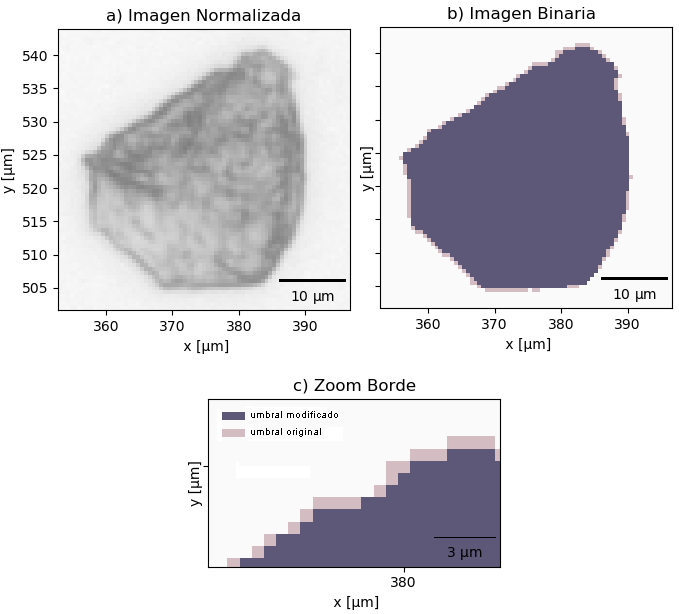
\includegraphics[scale=1.2]{Figs/cuantificaciondefectos/erroresborde.png}
\caption{\texttt{a)} Región de una imagen normalizada con un defecto.\texttt{b)} Imágenes binarias superpuestas del umbral original y de su variación para cuantificar el error cometido. \texttt{c)} Zoom sobre uno de los bordes del defecto.}
\label{fig:bordedefe}
\end{figure}

En el ejemplo de la Figura \ref{fig:bordedefe} se obtuvo un defecto con un área que para el umbral original estuvo compuesta por 2793 píxeles (959$\mu m^{2}$) y para su variación el área fue de 2640 píxeles (906$\mu m^{2}$). El diámetro equivalente fue de 35$\mu m$ y 34$\mu m$ respectivamente. En todos los resultados de diámetros y áreas de defectos detectados con el algoritmo explicado en la sección \ref{sec:secalg}, se reportó el resultado obtenido con el umbral original y se asoció como incerteza la diferencia entre el valor obtenido con el umbral y su variación. Así por ejemplo, el defecto de la Figura \ref{fig:bordedefe} tuvo un diámetro de $(35 \pm 1) \mu m$.

A continuación se describe la construcción y montaje del equipo desarrollado en la presente tesis para caracterizar espectralmente a los defectos definidos en este capítulo como agujeros ó huecos (Ver Figura  \ref{fig:huecoazul}) y manchas ó defectos de transmisión (Ver Figura \ref{fig:manchaazul}).

En el Capítulo 3 se realizó una descripción cuantitativa de los defectos: se determinó su tamaño, área, la cantidad de defectos presentes en cada banda. Este tipo de análisis de los defectos sigue la línea de las especificaciones técnicas de \textit{scratch \& dig} y la ISO 10110 en cuanto a que no realizan un análisis cualitativo de los defectos. En el presente trabajo se montó un microespectrómetro para caracterizar espectralmente los defectos. Esto es,


\vspace{1cm}
\todo[inline]{Eventualmente la seccion caracteristicas del filtro va en la introd?}
\vspace{1cm}



\vspace{1cm}
\todo[inline]{para poner el error del metodo en decir un defecto es de 15 mics $\pm$ poner el error del m[etodo triangle que le emboca a todos los defectos pero SOBREESTIMA el tamaño, los hace mucho más grandes..}
\vspace{1cm}


\vspace{1cm}
\todo[inline]{ small crater on the polished optical surface .. decir algo que los agujeros son lo que dice antes}
\vspace{1cm}



 \vspace{1cm}
\todo[inline]{en la seccion caracteristicas del filtro, en el itemize de las bandas..ver de explicar para qué sirve cada banda, usar por ej: \href{http://gspperu.com/pdf/res_landsat7etm.pdf}{link}}
\vspace{1cm}

\vspace{1cm}
\todo[inline]{si hace falta explicar un poco en que consisten los filtros opticos de interferencia..}   
\vspace{1cm}

\vspace{1.0cm}
\todo[inline]{explicar que tipo de lampara es la del Zeiss}
\vspace{1.0cm}

\vspace{1.0cm}
\todo[inline]{Cómo asociar errores a las dimensiones medidas tanto con el fiji como con el algoritmo. Al error de las imágenes del zeiss se le pone la calibración, por ej $\pm$ 0.586 $\mu$m , aprox 0.59 micrones de error }
\vspace{1.0cm}

\vspace{1cm}
\todo[inline]{hace falta explicar las cuentas de la normalizacion de las imagenes.. o que lean la cita de nordenfelt}   
\vspace{1cm}


\vspace{1cm}
\todo[inline]{estimacion de errores, ROI estimacion de falsos positivos falsos negativos tasa de error del sistema, por inspeccion visual nomas}
\vspace{1cm}


\vspace{1cm}
\todo[inline]{ver imagenes y cuantificar cuantos defectos de los mas chicos no agarra, se hace a ojo si o si, revisar banda completa tomando nota de defectos reales vs defectos encontrados y cuantificarlo de alguna manera}
\vspace{1cm}

\vspace{1cm}
\todo[inline]{diagrama de flujo para el algoritmo de deteccion}
\vspace{1cm}

\vspace{1cm}
\todo[inline]{explicar que tipo de lampara es, escuchar audio hernan, poner el codigo de github del espectro con colores facha}
\vspace{1cm}


\vspace{1cm}
\todo[inline]{Falta: poner siempre la barrita de la escala en las imágenes}
\vspace{1cm}














